\documentclass[11pt]{article}
\usepackage[a4paper]{geometry}
%\usepackage[T1]{fontenc}
\usepackage{lmodern,microtype,amsmath,amssymb,amsthm,mathtools,enumitem}
\usepackage{xcolor}
\usepackage{tikz}
\usepackage[colorlinks=true,linkcolor=blue,citecolor=blue,urlcolor=blue]{hyperref}
%\hypersetup{pdftitle={Coherence and Dominance under General Rankings},hypertexnames=false}


\newtheorem{theorem}{Theorem}[section]
\newtheorem{lemma}[theorem]{Lemma}
\newtheorem{proposition}[theorem]{Proposition}
\newtheorem{corollary}[theorem]{Corollary}
\newtheorem{conjecture}[theorem]{Conjecture}
\newtheorem{sublemma}{Sublemma}[theorem]
\theoremstyle{definition}
\newtheorem{definition}[theorem]{Definition}
\newtheorem{example}[theorem]{Example}
\theoremstyle{remark}
\newtheorem{remark}[theorem]{Remark}



\newcommand{\R}{\mathbb R}
\newcommand{\N}{\mathbb N}
\newcommand{\M}{\mathcal M}
\newcommand{\C}{\mathcal C}
\newcommand{\U}{\mathcal U}
\newcommand{\PP}{\mathcal P}
\newcommand{\G}{\mathcal G}
\newcommand{\Lf}{\mathfrak L}
\newcommand{\agenda}{\mathcal F}
\newcommand{\one}{\mathbf 1}
\newcommand{\supp}{\operatorname{supp}}
\newcommand{\Exp}{\operatorname{Exp}}
%\setlist{itemsep=1pt,topsep=3pt}

\title{Dominance Generalised}
\author{Jason Konek and Catrin Campbell-Moore}




%CCM added
\usepackage{cleveref}
\usepackage{stmaryrd}
\usetikzlibrary{arrows.meta}


\newcommand{\given}{\,:\,}


\newcommand{\FSP}{\mathrm{FSP}}
\newcommand{\FAP}{\mathrm{FAP}}
\newcommand{\closure}{\mathsf{closure}}


\newenvironment{AIwritten}{\begin{color}{blue}}{\end{color}}


\usepackage[textsize=footnotesize,obeyFinal,backgroundcolor=white,bordercolor=gray!20,linecolor=gray!20]{todonotes} % use "\PassOptionsToPackage{disable}{todonotes}" to disable in a document


\begin{document}
\maketitle

\section{Dominance Arguments}

We pin down certain ways of measuring goodness of objects in some class, $M$, at different points, usually at each possible world. So we have comparative relations $\succeq_w$ on $M$ for each $w$. We don't assume anything about the structure of these relations yet. 


A dominance argument will identify a flaw in certain kinds of members of $M$, when there is some alternative which is at least as good no matter what, and is somewhere better. 
%If $m$ is dominated, and the ranking which deems it so is a legitimate ranking, then $m$ is taken to be irrational. 
%If we merely identify a class of legitimate rankings and some objects are dominated on some rankings and not on others, there are differences that one can say about the rationality status, and this will depend on how we understand the various legitimate rankings to apply, but at least they don't have the 



In this paper we are not providing arguments for particular rankings but instead identifying a central tool for giving dominance arguments and the properties of the rankings which are required to obtain such a dominance result. It encompasses most of the applications of accuracy dominance results in the literature and hopefully pave the way for new applications. 

In particular, we highlight the merely instrumental role of strict propriety and replace it with something much more general involving dominance type considerations: finitely supported probabilities must not be dominated on their support. And we highlight how this parallel assumption is obtained in a whole class of applications where it is not credence functions themselves which are being evaluated. 


Since we usually identify rankings by spelling out axioms, we typically cannot pin down a unique ranking. 
If $m$ is dominated on every legitimate ranking, then it is flawed and irrational. What though about models whose status differs on different legitimate rankings? 
As defended in Konek, we will take them to be rational, at least they don't have this flaw. This does not play much of a role in the paper, as in most applications, all legitimate rankings agree about what the class of dominated models are. 


\section{Core result}



\subsection{Finite $W$}

\subsubsection{Preliminaries: Finitely Supported Probabilities}

\begin{definition}
For a finite nonempty set $W$,
\[
\Delta_W
:= \left\{p\in\mathbb{R}^W :
p(w)\geq 0 \text{ for all } w\in W,\quad
\sum_{w\in W}p(w)=1\right\},
\]
with the topology inherited from $\mathbb{R}^W$.

For $p\in \Delta$, $\operatorname{supp}(p):=\{w\in W:p(w)>0\}$
\end{definition}

These are probability mass functions. 

%
%Its vertices are the point masses $\delta_w$, one for each $w\in W$.
%
%For each nonempty $S\subseteq W$, the face spanned by the vertices
%indexed by $S$ is
%\[
%\operatorname{conv}\{\delta_w:w\in S\}
%= \{p\in\Delta_W:\operatorname{supp}(p)\subseteq S\},
%\]
%where $\operatorname{supp}(p)=\{w\in W:p(w)>0\}$.
%
%\begin{theorem}[KKM lemma]
%	Suppose $W$ is a finite nonempty set and
%	$\psi:W\rightrightarrows\Delta_W$ assigns a closed subset of
%	$\Delta_W$ to each $w\in W$. If
%	\[
%	\operatorname{conv}\{\delta_w:w\in S\}
%	\subseteq \bigcup_{w\in S}\psi(w)
%	\qquad\text{for every nonempty } S\subseteq W,
%	\]
%	then $\bigcap_{w\in W}\psi(w)$ is nonempty.
%\end{theorem}
%
%The face-covering condition is equivalent to requiring that for every
%$p\in\Delta_W$ there is some $w\in\operatorname{supp}(p)$ such that
%$p\in\psi(w)$. In one direction, apply the face-covering condition to
%$S=\operatorname{supp}(p)$. In the other direction, if $p$ lies in the
%face indexed by $S$, then $\operatorname{supp}(p)\subseteq S$, so any
%such $w$ belongs to $S$.
	

\subsubsection{Mathematical theorem}

The following is a version of the well-known Knaster–Kuratowski–Mazurkiewicz (KKM) lemma. We have stated it directly in terms of probabilities to already be closer to our inteded domain of applications. The proof that it follows from the standard KKM lemma, along with a statement of that, is in the appendix. 

\begin{theorem}[KKM]
	Suppose $W$ is a finite nonempty set.
	Suppose $\psi:W\rightrightarrows \Delta_W$ satisfies:\begin{itemize}
	\item \textbf{Closed} For every $w$, $\psi(w)$ is closed in $\Delta_W$
	\item \textbf{KKM covering} For every $p\in \Delta_W$, there is some $w\in\supp(p)$ such that $p\in\psi(w)$.
\end{itemize}
Then there is some $p\in \Delta_W$ such that for all $w\in W$, $p\in\psi(w)$. Moreover, the set of such $p$ is compact.
\end{theorem}

The KKM covering condition requiring that $w\in\supp(p)$ is very important. It requires, for example, that $\delta_w\in \psi(w)$.

\subsubsection{Application to dominance}

$\succeq_w$ is a relation on some set $M$ representing  ``at least as good as in $w$''.
the conclusion of the theorem says that for every model there is some special kind of object (those which are mapped to by the function $s$) which is guaranteed to be at least as good as it. 

%\begin{definition}
%	$m$ is dominated by $m'$ iff \begin{itemize}
%		\item for all $w\in W$, $m\succeq_w m'$, and
%		\item for some $w\in W$, $m'\not\succeq_w m$. 
%	\end{itemize}
%\end{definition}


\begin{corollary}
	Suppose $W$ is a finite nonempty set.
	
	Suppose $M$ is a nonempty set and $s:\Delta_W\to M$.
	Let $\succeq_w$ be a comparative relation on $M$ for each $w\in W$.
	
	If
	\begin{itemize}
		\item \textbf{Closed} For every $m\in M$ and $w\in W$,
		\[
		\{p\in\Delta_W\given s(p)\succeq_w m\}
		\]
		is closed in $\Delta_W$.
		
		\item \textbf{KKM covering} For every $p\in\Delta_W$ and
		$m\in M$, there is some $w\in\supp(p)$ such that
		\[
		s(p)\succeq_w m.
		\]
	\end{itemize}
	Then for every $m\in M$, there is some $p\in\Delta_W$ such that
	\[
	s(p)\succeq_w m
	\text{ for every }w\in W.
	\]
	Moreover, the set of such $p$ is compact.
	
	If $R\subseteq M$ is such that
	\begin{itemize}
		\item $s(\Delta_W)\subseteq R$ and
		\item There can be no everywhere-ties between members of $R$
		and those outside of $R$:\footnote{This is like the quasi
			propriety type weakening of Pruss, or is it Nielson?} \\
		If $r\in R$ and $m\in M\setminus R$, and for all $w$
		$m\succeq_w r$, then there is some $w$ such that
		$r\not\succeq_w m$.
	\end{itemize}
	then members outside of $R$ must be dominated.
	
	If, in addition,
	\begin{itemize}
		\item the objects in $R$ cannot be dominated
	\end{itemize}
	then $m$ is in $R$ iff it is undominated, and those that are
	not in $R$ are dominated by something which is undominated.
\end{corollary}

\begin{proposition}[Sufficient conditions for KKM covering]
		If $\succeq_w$ is total, the KKM covering is just to say that for all probabilities $p$, there is no model which is $p$-surely strictly better than $s(p)$.		
		
		If $\succeq_w$ is generated by a loss function, then this follows from weak $s$-propriety: 
		for every $p$, $\Exp_p[\l(s(p))]\geq\Exp_p[\l(m)]$. 
	
		
		It would also follow from other evaluation functions, such as risk-weighted expectations, so long as they have the following respecting dominance type property: 
		\begin{itemize}
			\item For $p\in\Delta$, if $E_p[X]\geq E_p[Y]$ then there is some $w\in\supp(p)$ such that $X(w)\geq Y(w)$.
			\item If it's all totally ordered:\\
			For fs $p$, If $X(w)< Y(w)$ for all $w\in\supp(p)$, then $E_p[X]<E_p[Y]$. 
		\end{itemize}
		
		If the loss function is \emph{strictly} $s$-proper, then putting $R=s(\Delta)$, we get everything in the theorem except closure. 
\end{proposition}

\begin{proposition}[Sufficient condition for Closed]
	If $\succeq_w$ is generated by a loss function, then \textbf{Closed} holds if $p\mapsto L(s(p),w)$ is continuous, or even lower semicontinuous. For example, because $M$ is endowed with a topology on which $s$ is continuous and $L(\cdot,w)$ is also continuous for each $w$.  
\end{proposition}





\begin{color}{violet}
	
	
	\begin{AIwritten}
		\begin{corollary}
			Suppose $W$ is a finite nonempty set.
			
			Suppose $M$ is a nonempty set, $R\subseteq M$, and
			$s:\Delta_W\to M$ satisfies $s(\Delta_W)\subseteq R$.
			Let $\succ_w$ be a strict comparative relation on $M$ for
			each $w\in W$.
			
			If
			\begin{itemize}
				\item \textbf{Open} For every $m\in M\setminus R$ and $w\in W$,
				\[
				\{p\in\Delta_W\given s(p)\succ_w m\}
				\]
				is open in $\Delta_W$.
				
				\item \textbf{KKM covering} For every $p\in\Delta_W$ and
				$m\in M\setminus R$, there is some $w\in\supp(p)$ such that
				\[
				s(p)\succ_w m.
				\]
			\end{itemize}
			Then for every $m\in M\setminus R$, there is some
			$p\in\Delta_W$ such that
			\[
			s(p)\succ_w m
			\text{ for every }w\in W.
			\]
			
			If, in addition,
			\begin{itemize}
				\item the objects in $R$ cannot be strictly dominated,
			\end{itemize}
			then $m$ is in $R$ iff it is not strictly dominated, and every
			$m$ outside $R$ is strictly dominated by something that is
			itself not strictly dominated.
		\end{corollary}
		
		\begin{proof}
			Fix $m\in M\setminus R$ and put
			\[
			U_w=\{p\in\Delta_W\given s(p)\succ_w m\}.
			\]
			The $U_w$ are open and satisfy the KKM covering condition.
			By the open-set version of KKM, there is some
			$p\in\bigcap_{w\in W}U_w$. Thus $s(p)\in R$ strictly
			dominates $m$. The final claim follows from the additional
			assumption on $R$.
		\end{proof}
	\end{AIwritten}
\end{color}

\subsubsection{Generalisations}
\begin{theorem}
	The selection $s(p)$ can depend on the fixed model we are considering, $m^*$: $s_{m^*}(p)$
\end{theorem}
%This is useful, for example, when the space which is being considered is unbounded. (E.g.~Wald). 

In \cref{thm:dom} we let $\psi_{m^*}(w)=\{p\in P:s(p)\succeq_w m^*\}$. We could have instead selected $\psi_{m^*}$ to be closed subsets of this, so long as the KKM covering condition still holds. 
\begin{theorem}
	The conclusion of \cref{thm:dom} holds if we can select sets $\psi_{m^*}(w)\subseteq P$ which satisfy the conditions of \cref{thm:KKM} such that for every $w$, $\psi_{m^*}(w)\subseteq\{p: s(p)\succeq_w m^*\}$. 
\end{theorem}

\begin{theorem}
	The selection $s$ may also be a nonempty-valued
	correspondence. In that case, define
	\[
	\psi_{m^*}(w)
	=
	\{p:\text{every }m\in s(p)
	\text{ satisfies }m\succeq_w m^*\}.
	\]
	If these sets are closed and satisfy the KKM covering
	condition, then there is some $m$ (take any in $s(p)$) which is at least as good as $m^*$ at every world.
\end{theorem}

%\begin{theorem}
%	The set $P$ can be any compact Hausdorff space
%	containing $\mathrm{FSP}(W)$, such that the inclusion
%	$\Delta_F\hookrightarrow P$ is continuous for
%	every nonempty finite $F\subseteq W$.
%\end{theorem}
%\begin{theorem}
%	Suppose $P$ is a compact Hausdorff topological space, and $\iota:\mathrm{FSP}(W)\to P$ continuous on each finite $\Delta_F\subseteq\mathrm{FSP}(W)$. 
%	
%	Suppose there is $s\colon P\to M$ such that:
%	\begin{enumerate}
	%		\item\label{ass:cl} \textbf{Closedness.}
	%		For every $m^* \in M$ and $w \in W$, the set
	%		\[
	%		\{p\in P\given s(p)\succeq_w m^*\}
	%		\]
	%		is closed in $M$.
	%		
	%		\item \label{ass:KKM}\textbf{KKM covering.}
	%		For every finitely supported $p \in \mathrm{FSP}(W)$ and every
	%		$m \in M$, 
	%		%		$s(p)$ is at least as good as $m$ at some $w\in\supp(p)$: 
	%		there is some $w \in \operatorname{supp}(p)$
	%		such that
	%		\[
	%		s(\iota(p)) \succeq_w m.
	%		\]
	%	\end{enumerate}
%	Then, for every $m \in M$, there exists some $p\in P$ such that:
%	\[
%	s(p) \succeq_w m
%	\qquad \text{for every } w \in W.
%	\]
%	The set of such $p$ is also compact. 
%\end{theorem}
%\begin{proof}
%	content...
%\end{proof}


\subsection{Infinite $W$}


\subsubsection{Preliminaries: Finitely Supported Probabilities}
\begin{definition}
Let $W$ be a nonempty set. For $p\in[0,1]^W$, define
$$\operatorname{supp}(p):=\{w\in W:p(w)>0\}$$ The set of finitely
supported probabilities on $W$ is
\[
\mathrm{FSP}
:= \left\{p\in[0,1]^W \;\middle|\;
\operatorname{supp}(p)\text{ is finite and }
\sum_{w\in\operatorname{supp}(p)}p(w)=1
\right\}.
\]

For each finite nonempty $F\subseteq W$, let $\Delta_F$ be the simplex
of probabilities supported in $F$:
\[
\Delta_F
:= \{p\in\mathrm{FSP}:\operatorname{supp}(p)\subseteq F\}.
\]
Restriction to $F$ identifies $\Delta_F$ with the standard simplex
$\{q\in[0,1]^F:\sum_{w\in F}q(w)=1\}$. We equip $\Delta_F$ with
the Euclidean topology under this identification. With $\Delta_F$
defined as a subset of $\mathrm{FSP}$, we have
\[
\mathrm{FSP}
= \bigcup_{\substack{\varnothing\ne F\subseteq W\\ F\text{ finite}}}
\Delta_F.
\]
\end{definition}

\subsubsection{Mathematical theorem}

Using compactness, the following extension of the KKM result applies in infinite settings:
\begin{theorem}
	Suppose $W$ is a nonempty set, and $\Theta$ is a compact space with $\sigma:\FSP\to \Theta$ continuous on each $\Delta_F$. 
	
	Suppose $\psi:W\rightrightarrows \Theta$ satisfies:\begin{itemize}
		\item \textbf{Closed} For every $w$, $\psi(w)$ is closed in $\Theta$
		\item \textbf{KKM covering} For every $p\in \FSP$, there is some $w\in\supp(p)$ such that $p\in\psi(w)$.
	\end{itemize}
	Then there is some $\theta\in\Theta$ such that for all $w\in W$, $\theta\in\psi(w)$. Moreover, the set of such $\theta$ is compact.
\end{theorem}
\begin{proof}
	Fix a finite $F\subseteq W$, consider $\phi:F\rightrightarrows \Delta_F$ with $\phi(w)=\sigma^{-1}(\psi(w))=\{p\in\Delta_F\given \sigma(p)\in\psi(w)\}$. By continuity of $\sigma$, this is closed. And has the KKM covering property.  So there is some $p$ such that $\sigma(p)\in\psi(w)$ for all $w\in F$. This gives some $\theta\in \bigcap_{w\in F}\psi(w)$. 
	
	Thus, $\{\psi(w)\given w\in W\}$ is a collection of closed sets with the finite intersection property, and so has non-empty intersection by compactness. 
\end{proof}

\subsubsection{Application to dominance results}



\begin{center}
	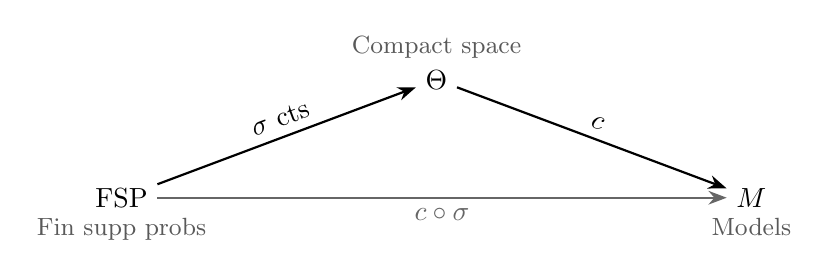
\begin{tikzpicture}[
		map/.style={-{Stealth}, thick},
		caption/.style={font=\small, text=black!65}
		]
		
		\node (fsp) at (0,0) {$\FSP$};
		\node (theta) at (4,1.5)
		{$\Theta$};
		\node (m) at (8,0) {$M$};
		\node[caption, below=4pt] at (fsp)
		{Fin supp probs};
		\node[caption, above=4pt] at (theta)
		{Compact space};
		\node[caption, below=4pt] at (m)
		{Models};
		
		\draw[map] (fsp) -- node[above, sloped]
		{$\sigma$ cts} (theta);
		\draw[map] (theta) -- node[above, sloped]
		{$c$}  (m);
	\draw[map,black!60] (fsp) -- node[below]
{$c\circ \sigma$}  (m);
		
	\end{tikzpicture}
\end{center}

\begin{corollary}
	Suppose $W$ is a nonempty set, and $\Theta$ is a compact space with $\sigma:\FSP\to \Theta$ continuous on each $\Delta_F$. 
	
	Suppose $M$ is a nonempty set and $c:\Theta\to M$. We have $\succeq_w$ is a comparative relation on a nonempty set $M$, for each $w\in W$. 
	
	If \begin{itemize}
		\item \textbf{Closed} For every $m\in M$ and $w$, \[\{\theta\in\Theta\given c(\theta)\succeq_w m\}\] is closed
		\item \textbf{KKM covering} For every $p\in \FSP$ and $m\in M$, there is some $w\in\supp(p)$ such that $$c(\sigma(p))\succeq_w m$$
	\end{itemize}
	Then there is some $\theta\in\Theta$ such that 
	\[
	c(\theta)\succeq_w m
	\text{ for every }w\in W
	\] 
	Moreover, the set of such $\theta$ is compact.

	If $R\subseteq M$ is such that:
	\begin{itemize}
		\item $c(\Theta)\subseteq R$ and
		\item There can be no everywhere-ties between members of $R$ and those outside of $R$:\footnote{This is like the quasi propriety type weakening of Pruss, or is it Nielson?} \\
		If $r\in R$ and $m\in M\setminus R$, and for all $w$ $m\succeq_w r$, then there is some $w$ such that $r\not\succeq_w m$.
	\end{itemize}then members outside of $R$ must be dominated. 
	
	If, in addition, \begin{itemize}
		\item the objects in $R$ cannot be dominated
	\end{itemize} then $m$ is in $R$ iff it is dominated, and those that are not in $R$ are dominated by something which is not itself dominated. 
\end{corollary}

Propriety is used to get KKM covering. Importantly, then, we see that it is only needed for finitely-supported probabilities. 



\subsubsection{Version via $M$}



One version of this theorem is to identify $\Theta$ with a subspace of $M$. This requires $M$ to have a topology and $s:\FSP\to M$, and $\closure(s(\FSP))$ is compact. 

\begin{center}
	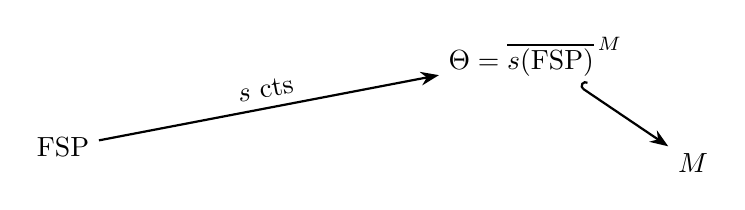
\begin{tikzpicture}[
		map/.style={-{Stealth}, thick},
		inclusion/.style={{Hooks[right]}-{Stealth}, thick},
		caption/.style={font=\small, text=black!65}
		]
		
		% (1) Compact closure in M
		\node (fsp1) at (0,0) {$\FSP$};
		\node (theta1) at (6,1.15)
		{$\Theta=\overline{s(\FSP)}^{\,M}$};
		\node (m1) at (8,-.2) {$M$};
		
		\draw[map] (fsp1) -- node[above, sloped]
		{$s$ cts} (theta1);
		\draw[inclusion] (theta1) -- (m1);
		
	\end{tikzpicture}
\end{center}


\begin{corollary}
	Suppose $W$ is a nonempty set. Suppose $M$ is a topological space.
	
	Suppose $\succeq_w$ is a comparative relation on a nonempty set $M$, for each $w\in W$. 
	
	And suppose $s:\FSP\to M$ is continuous on each finite $\Delta_F$. Let $$\Theta=\overline{s(\FSP)}^{\,M}$$
	
	If \begin{itemize}
		\item \textbf{Closed} For every $m\in M$ and $w$, \[\{\theta\in\Theta\given \theta\succeq_w m\}\] is closed in $\Theta$, or $M$.
		\item \textbf{KKM covering} For every $p\in \FSP$ and $m\in M$, there is some $w\in\supp(p)$ such that $$s(p)\succeq_w m$$
	\end{itemize}
	Then there is some $\theta\in\Theta$ such that 
	\[
	\theta\succeq_w m
	\text{ for every }w\in W
	\] 
	Moreover, the set of such $\theta$ is compact.
	
	If $R\subseteq M$ is such that:
	\begin{itemize}
		\item $\Theta\subseteq R$ and
		\item There can be no everywhere-ties between members of $R$ and those outside of $R$:\footnote{This is like the quasi propriety type weakening of Pruss, or is it Nielson?} \\
		If $r\in R$ and $m\in M\setminus R$, and for all $w$ $m\succeq_w r$, then there is some $w$ such that $r\not\succeq_w m$.
	\end{itemize}then members outside osf $R$ must be dominated. 
	
	If, in addition, \begin{itemize}
		\item the objects in $R$ cannot be dominated
	\end{itemize} then $m$ is in $R$ iff it is dominated, and those that are not in $R$ are dominated by something which is not itself dominated. 
\end{corollary}

\subsubsection{Version via embedding $\FSP$ in a compact space}

Another version is where we take $\Theta$ to itself be a compact space including $\FSP$. This can either be the space of finitely additive probabilities or the space of linear previsions for bounded gambles, or the space of exteded-valued linear previsions for unbounded gambles. Then $s:\Theta\to M$. Note that it cannot be the sigma-additive probabilities, as this is not compact. 


\begin{center}
	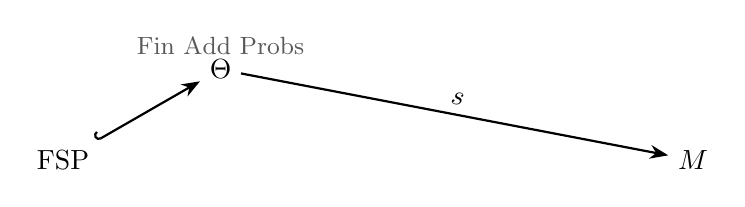
\begin{tikzpicture}[
		map/.style={-{Stealth}, thick},
		inclusion/.style={{Hooks[right]}-{Stealth}, thick},
		caption/.style={font=\small, text=black!65}
		]
		
		% (2) Compactification of FSP
		\node (fsp2) at (0,-2.4) {$\FSP$};
		\node (theta2) at (2,-1.25) {$\Theta$};
		\node[caption, above=2pt] at (theta2)
		{Fin Add Probs};
		\node (m2) at (8,-2.4) {$M$};
		
		\draw[inclusion] (fsp2) -- node[above, sloped] {} (theta2);
		\draw[map] (theta2) -- node[above, sloped] {$s$} (m2);
	\end{tikzpicture}
\end{center}


\begin{corollary}\label{thm:FAP}
	Suppose $W$ is a nonempty set, and $\Theta$ is a compact space with $\sigma:\FSP\to \Theta$ continuous on each $\Delta_F$. Suppose that $\sigma$ is injective. We identify each $p\in \FSP$ with a member of $\Theta$. 
	
	Suppose $M$ is a nonempty set and $s:\Theta\to M$. We have $\succeq_w$ is a comparative relation on a nonempty set $M$, for each $w\in W$. 
	
	If \begin{itemize}
		\item \textbf{Closed} For every $m\in M$ and $w$, \[\{\theta\in\Theta\given s(\theta)\succeq_w m\}\] is closed
		\item \textbf{KKM covering} For every $p\in \FSP$ and $m\in M$, there is some $w\in\supp(p)$ such that $$s(p)\succeq_w m$$
	\end{itemize}
	Then there is some $\theta\in\Theta$ such that 
	\[
	s(\theta)\succeq_w m
	\text{ for every }w\in W
	\] 
	Moreover, the set of such $\theta$ is compact.
	
	If $R\subseteq M$ is such that:
	\begin{itemize}
		\item $s(\Theta)\subseteq R$ and
		\item There can be no everywhere-ties between members of $R$ and those outside of $R$:\footnote{This is like the quasi propriety type weakening of Pruss, or is it Nielson?} \\
		If $r\in R$ and $m\in M\setminus R$, and for all $w$ $m\succeq_w r$, then there is some $w$ such that $r\not\succeq_w m$.
	\end{itemize}then members outside of $R$ must be dominated. 
	
	If, in addition, \begin{itemize}
		\item the objects in $R$ cannot be dominated
	\end{itemize} then $m$ is in $R$ iff it is dominated, and those that are not in $R$ are dominated by something which is not itself dominated. 
\end{corollary}

\subsubsection{Relation to the finite result}

If $W$ is finite, then this reduces to the special case, putting $\Theta=\FSP$, which is clearly compact, and $s:\FSP\to M$.

\begin{center}
	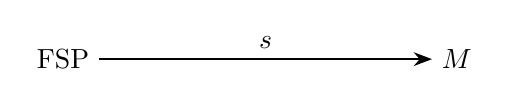
\begin{tikzpicture}[
		map/.style={-{Stealth}, thick},
		inclusion/.style={{Hooks[right]}-{Stealth}, thick},
		caption/.style={font=\small, text=black!65}
		]
		
		% (2) Compactification of FSP
		\node (fsp2) at (0,-2.4) {$\FSP$};
		\node (m2) at (5,-2.4) {$M$};
		
		\draw[map] (fsp2) -- node[above, sloped] {$s$} (m2);
	\end{tikzpicture}
\end{center}


\part{Applications}
Our different applications are simply identifying particular $M$ and criteria on the ordering which imply the existence of a suitable $s$ supporting a dominance argument for various rationality criteria. 

\section{Core application: dominance argument for probabilistic coherence.}




%\subsection{Dominance argument for probabilistic coherence}

Here we are judging credence functions. 
Fix $W$ and let $\agenda\subseteq W$. 
$$M=\R^\agenda$$

Alternatively, we might take $\agenda$ to be a set of sentences, with $\llbracket \phi\rrbracket \subseteq W$.

\begin{definition}
	$p\in \R^{\wp(W)}$ is a finitely additive probability function if \ldots.
\end{definition}
\begin{lemma}
	$\FAP$ is a compact space including $\FSP$, so we will make use of \cref{thm:FAP}
\end{lemma}

There is a natural $s:\FAP\to M$ where $$s(p)(A)=p(\llbracket A\rrbracket)$$

\begin{definition}
	$c\in \R^\agenda$ is probabilistic if there is a finitely additive probability $p\in \FAP$ such that $c=s(p)$. 
	
	Let $R\subseteq M$ be the collection of probabilistic credence functions, that is $R=s(\FAP)$. 
\end{definition}

\begin{proposition}
	If comparative evaluation is generated by a quasi-proper scoring rule which is continuous, then all the conditions of the theorems are satisfied. We thus have that non-probabilities are strictly dominated by probabilities, which are themselves not even weakly dominated. 
\end{proposition}

Propriety goes well-beyond the KKM conditions. They are only interested in dominance, albeit dominance on the support of $p$. This also means that the same would hold if we use other evaluation functions than expectations. For example, if we use a risk-weighted quasi-proper loss function exactly the same argument would go through. 



\section{Dominance argument for convex hulls}
\subsection{Credence functions in non-classical logic}

We could also consider non-classical probability functions. Now $W$ are the possible points of evaluation, associated with omniscient credence functions which need not satisfy the classical laws of probability, and $s(p)$ is a $p$-weighted average of the omniscient points. 

$v_w\in M$ be an ``omniscent model'' at world $w$. 

Williams argues that what we get is a dominance argument for being in the convex hull of the omniscient points. 

This is right, when the measure has the properties of the $p$-weighted averages being not $p$-dominated. For example, when it is appropriately proper. 

Williams applies this where $M=\R^{Sent}$ too. 
But it could also apply where, for example, each sentence obtains two real values, as is argued for in Janda. It works in any Hausdorff topological vector space. 

We get an argument for being in the closure of the convex hull of the omniscint models, which works so long as this is a compact set. 

\subsection{Deference to Chance}

Take the ``worlds'' to be objective chance functions. But the objects being evaluated are still credence functions, involving worlds. Again we have an argument for being in the closure of the convex ull of the objective chance functions. 

\section{Estimation as expectation}

Observation: for this section we can easily use either of the theorems. We can use the closure of the convex hull. Or we can take $\Theta$ to be the independent space consisting of these. 

To encompass the risk-weighted ones, 


\subsection{Bounded gambles}

\subsection{Unbounded gambles}

\subsection{Risk-weighted expectations}

Map finitely supported probabilities to risk-weighted expected values. 
The closure of this is compact (since it's a closed subset of a compact space). 

So the theorem would apply. This depends, though, on whether one's ranking evaluates risk-weighted or the straight-up expectations to be the objects which are not dominated on the support. 




\section{Conditionalisation}

This is quite different to the others: there's no single obvious characterisation of $s(p)$ when some $p(E)=0$. Moreover, converging to probability $0$ from different directions can result in different required posteriors. 

We will describe a continuous $s$ mapping each $p$ to a conditionalisation plan, but not a conditionalisation plan for $p$ itself, but for a different prior, one which assigns probability 0 to more events than $p$ does, ones below a threshold. 

\newpage\color{red}




\subsection{Dominance argument for probabilistic coherence}


Suppose $M$ is a class of models which in fact contains probabilities directly. For example, it is the space of credence functions defined on the whole $\wp{W}$. And suppose $\succeq_w$ is an ordering on $M$ for each $w$. 
\begin{proposition}
	Suppose $P\subseteq\M$ and $\succeq_w$ is an ordering on $\M$ such that:
	\begin{itemize}
		\item For all models $m$, $\{p\text{ probability} : p\succeq_w m\}$ is closed. 
		\begin{itemize}
			\item For example, each $\succeq_w$ is generated by a continuous (or lower semi-continuous) loss function.
		\end{itemize}
	\item For all fs probs $p$ and models $m$, there is some $w\in\supp(p)$ in which $p$ is at least as good as $m$. 
		\begin{itemize}
			\item If $\succeq_w$ are total, this is to say that for fs probs there is no $m$ which is $p$-surely strictly better than $p$: fs probs are not strictly dominated on their support. 
		\end{itemize}
	\end{itemize}
	Then non-probabilities are Pareto-dominated by, or have the same loss profile as, a probability function. 
	
	If, in addition, 
	\begin{itemize}
		\item there can be no probabilistic $p$ and non-prbabilistic $m$ which are tied at every world
	\end{itemize}
	Then in fact, every non-probability is Pareto-dominated. 
	
	If, in addition, \begin{itemize}
		\item Probability functions are not dominated. 
	\end{itemize} Then we know that something is dominated iff it is non-probabilistic. And if it is probabilistic, then it is dominated by something which is not itself dominated. 
\end{proposition}
\begin{proof}
	Just let $s(p)=p$ and we have exactly the conditions. 
\end{proof}

%Let's describe some other sufficient conditions for the KKM
%\begin{lemma}
%	If $\succeq$ is a total ordering, then the KKM condition can be replaced with:
%	\begin{itemize}
%		\item  For all finitely additive probs, there is no model $m$ which is $p$-surely better than $p$. \\
%		That is, $p$ is not strictly dominated on its support. 
%	\end{itemize}
%\end{lemma}

Now, this KKM condition obviously follows from, for example, weak propriety: for every finitely additive probability $p$, $\Exp_p[\l(p)]\geq\Exp_p[\l(m)]$. It would also follow from other evaluation functions, such as risk-weighted expectations, so long as they have the following respecting dominance type property: 
	\begin{itemize}
	\item For fs $p$, if $E_p[X]\geq E_p[Y]$ then there is some $w\in\supp(p)$ such that $X(w)\geq Y(w)$.
	\item If it's all totally ordered:\\
	For fs $p$, If $X(w)< Y(w)$ for all $w\in\supp(p)$, then $E_p[X]<E_p[Y]$. 
\end{itemize}
Note that it's only for the finitely supported ones. Even standard Expected value doesn't satisfy this for \emph{all} fa probs: Bayes options can still be strictly dominated (atlhgough not uniformly dominated), but it does for the fs ones. 

So we also know that $r$-proper continuous functions are sufficient for a dominance argument for probabilism. 


%
%\begin{lemma}The following are sufficient for the covering part:
%	
%	Suppose $\succ_w$ is total.
%	
%	For all finitely supported probability functions, there is no model $m$ which is $p$-surely better than $c(p)$. That is, $p$ is not strictly dominated $\underline{on its support}$
%	
%	Suppose $\succ_w$ is generated by $\l:\M\times\Omega\to \R\cup\{\infty\}$.
%	$\l$ is weakly proper on finitely additive probabilities. That is, for every finitely additive probability $p$, $\Exp_p[L(p)]\geq\Exp_p[L(m)]$. 
%	
%	That's because this entails that there is some $w\in \supp(p)$ such that $L(p,w)\leq L(m,w)$. 
%	
%	In fact, other more general evaluation functions, such as risk-weighted expected values, would equally work, so long as they have this property: $E$ is a \emph{sensible evaluation} when:
%	\begin{itemize}
%		\item If $p$ is finitely additive and $E_p[X]\geq E_p[Y]$ then there is some $w\in\supp(p)$ such that  $X(w)\geq Y(w)$.
%	\end{itemize}
%	
%	Then, we ask that $\Lf$ be weakly $E$-proper on finitely additive probabilities. 
%\end{lemma}

Note that the condition that the world be in the support of $p$ is substantive and important. Simply imposing a simple form of Joyce's Coherent Admissibility is not sufficient: 
\begin{itemize}
	\item All fs probability functions are not strictly dominated. 
\end{itemize}
If $\delta_w$ is not strictly dominated because $\delta_w\succeq_{w^*}m$, but $\delta_w\prec_w m$, then the conditions are not satisfied. Being not dominated on the support requires that $\delta_w$ is optimal, with $\delta_w\succeq_w m$ for all $m\in M$. 

%\subsection{Evaluated objects don't include probabilities}
%Often what we are evaluating aren't themselves probabilities. 

\subsubsection{Infinite $\Omega$}
\todo[inline]{Make clear the difference between $\Omega$ infinite and infinite $\agenda$. Having this section here confuses it?}
Note that there is no restriction in this theorem to the space of possible outcomes, $\Omega$, being finite. 

The difficulty is, however, when there are infinitely many components of a credence function which need to be evaluated, that is, when the space of propositions over which the credence functions are defined is infinite, that is, when its domain is infinite. 

There are known challenges with applying accuracy considerations on arbitrary domains. It is impossible to get a real valued loss function which is strictly proper: there are just too many coherent models to expect comparisons to be reflected in the reals. This challenge has been made easier as we direclty work with orderings rather than real-valued loss functions. 

%Note that if the ordering satisfies ?? properties, then it is reflected by a loss function onto a field, and if it also satisfies Archimeanicity, it can be seen as a real-valued loss function. 

There is an outstanding question, however: for an arbitrary $\Omega$, is there a ranking which has the properties for the application of the theorem.
Yes, and trivially so: we could just use a loss function giving $0$ at every world to those which are theselves probabilities, and $1$ to those which are not. What's interesting is if it satisfies other desirable properties such as truth-directedness. For example, Snow Zhang shows that there are no comparative relations which are strictly truth directed and strongly extensional. 

\begin{remark}
	Let $c_1\succeq_wc_2$ iff $c_1\succeq_w^Fc_2$ for finite $F\subseteq \agenda$. 
	And suppose each $\succeq_w^F$ is continuous and strictly proper, for example, it's Brier score. 
	
	Take any $p$ and $c$. 	Is $\{p \given p\succeq_w c\}$ closed? Yes, I believe so. 
%	Suppose $p_\alpha$ is a net of probabilities with each $p^\alpha\succeq_w c$. That is, on every finite
	
	
	We want to find some $w$ where $p\succeq_w c$. 	This requires some $w$ such that for all $F$, $p\succeq_w^F c$. That's tantamount to saying that at world $w$ $p$ is at least as good as $c$ on every proposition. Switch of quantifiers. 
	
\end{remark}

Note also that it strengthens the theorem of Nielson \todo{does it??}

\subsubsection{Strict Dominance}
\todo[inline]{Move to end?}
That merely obtains Perato-dominance of the non-probabilities. The standard conclusion of the accuracy argument is that they are \emph{strictly} dominated. 

Some Bregman type stuff involved in the proof. Here we really do use something like propriety (although risk would do too); and probably it depends on finitely many worlds. 

\begin{theorem}
	If $\l$ is weakly proper and lower semi-continuous, then non-probabilities are at best tied with some probability; and if it is quasi-strictly proper then non-probabilities are uniformly-dominated. 
\end{theorem}
\begin{proof}
	Fix non-probability $m$. 
	
	Define \[D_m(p)=E_p[\l(m)]-E_p[\l(p)]\]
	
	This is everywhere strictly positive, by strict propriety, and is lower semicontinuous.\todo{justify}
	Since $P$ is compact, $D_m$ obtains its infimum on $P$, so we have $p^*\in P$ with 
	\[
	\nu=D_m(p^*)=\min_{p\in P}D_m(p)>0.
	\]
	
	
	We will show that $\l(m,w)\geq  \l(p^*,w)+\nu$ for all $w$
	
	
	For each world $w$, define
	\[
	\psi_m(w)=
	\{p\in P:\l(p,w)\le \l(m,w)-\nu\}.
	\]
	These sets are closed by lower semicontinuity.
	
	For every fs $p$
	\[D_m(p)=E_p[\l(m)]-E_p[\l(p)]=
	\sum_{w\in\supp(p)}
	p(w)\bigl[\l(m,w)-\l(p,w)\bigr]\ge\nu.
	\]
	Hence, for some $w\in\supp(p)$ we have \[\l(m,w)-\l(p,w)\ge\nu.
	\] that is, $p\in \psi_m(w)$. 
	This is the KKM covering condition.
	
	Fan--KKM supplies
	$p^*\in\bigcap_{w\in W}\psi_m(w)$,
	giving the stated uniform improvement.
	
\end{proof}
	\begin{remark}
	The argument also works with evaluations other
	than ordinary expectation. It suffices that they
	are translation invariant, respect comparisons
	on finite supports, and vary continuously with
	the probability for each random variable. 
	Propriety must then be understood relative to
	those evaluations. See Appendix~\ref{app:evaluations}.
\end{remark}




\subsection{Credence functions on any agenda}

Often we are not evaluating credence functions which have an opinion about every possible event. Instead they are defined as $c:\agenda\to\R$, where $\agenda$ is some subset of $\wp(W)$. It could also be not conceived of as events, subsets of $W$, but instead sentences in some language, which are satisfied in some worlds, so describe a subset of $W$.

We now just make the dual role of $P$ clear: they are probabilities over $W$, but what is evaluated are different: credence functions, which have a close connection to probabilities over $W$. 

There is then important content in the selection function $s:P\to M$. 

There is a very natural $s$ to use here: $s(p)(A)=p(A)$ for all $A\in \agenda$; or in the sentence formalism, $s(p)(\phi)=p(\llbracket \phi\rrbracket)$. \todo[inline]{there's something nice about the sentence formalism that we need to explicitly refer to $s$. I think we should use that case!}


Suppose $W$ is a nonempty set and $M=[0,1]^\agenda$ for some $\agenda\subseteq \wp(W)$.

\begin{definition}
	$c$ is probabilistic iff there is some probabilistic $p$ on $\wp(W)$ with $c=s(p)$. 
\end{definition}

\begin{proposition}
	Suppose $\succeq_w$ is an ordering on $\M$ such that:
	\begin{itemize}
		\item For all models $m$, $\{c\text{ probability} : c\succeq_w m\}$ is closed. 
		\begin{itemize}
			\item For example, each $\succeq_w$ is generated by a continuous (or lower semi-continuous) loss function.
		\end{itemize}
		\item For all $m$ and all $c$, if $p$ is finitely supported probability such that $s(p)=c$, then there is $w\in \supp(p)$ such that $c\succeq_w m$.
		\begin{itemize}
			\item If $\succeq_w$ are total, this is to say that the finitely supported probability functions give credence functions which are not almost-surely strictly dominated (on the support of the probability function). 
		\end{itemize}
	\end{itemize}
	Then non-probabilities are Pareto-dominated by, or have the same loss profile as, a probabilistic credence function. 
	
	If, in addition, there can be no probabilistic $p$ and non-prbabilistic $m$ which are tied at every world, then in fact, every non-probability is Pareto-dominated. 
\end{proposition}



\subsection{Non-classical probabilism}
We could also consider non-classical probability functions. Now $W$ are the possible points of evaluation, associated with omniscient credence functions which need not satisfy the classical laws of probability, and $s(p)$ is a $p$-weighted average of the omniscient points. 

$v_w\in M$ be an ``omniscent model'' at world $w$. 

Williams applies this where $M=\R^{Sent}$ too. But it could also apply where, for example, each sentence obtains two real values, as is argued for in Janda. It works in any Hausdorff topological vector space. 

What we're going to get out is a accuracy dominance argument for being in the convex hull of the omniscient models. 

This is delicate, however, once $W$ can be infinite, in which case we would only obtain a dominance argument for being in the closure of the convex hull of the omniscient models. This might not itself be compact if the omniscient points are unbounded in $M$ (assuming $M$ is locally compact), resulting in issues defining expectations. 

\todo[inline]{This is now so general it seems to encompass the linear previsions stuff. Too general? I want to apply it to the upper-lower pairs, but that's sich a simple application for this super generality. }

\begin{theorem}
	Suppose $M$ be a complete Hausdorff locally convex vector space. 
	
	Let $v_w\in M$ be an ``omniscent model'' at world $w$. 
	
	Suppose that $W$ is finite, or that the closure of $\{v_w\given w \in W\}$ is compact (in most real product spaces this is just requiring the set of omniscint models to be bounded in each coordinate.)
	
	Let $s(p):=\sum_w p(w) v_w$ for finitely supported $p$, well defined by the vector space structure of $M$.
	\todo{I'm just copying the general stuff!}
	If \begin{itemize}
		\item For every $m$ and every $w$, $\{p\given s(p)\succeq_w m\}$ is closed. \begin{itemize}
			\item For example it is generated by a lower semi-continuous loss function on models. 
		\end{itemize}
		\item For every $m$ and every fs $p$, there is some $w\in\supp(p)$ such that $s(p)\succeq_w m$. 
	\end{itemize}
\end{theorem}
\begin{proof}
	We use the parameter space $C:=closure(\{convexhull(\{omniscients\})\})$. It is compact 
\end{proof}
This is for example obtained by a version of propriety: For every fs $p$, $\Exp_p[L(m)]$ is minimised at $m=s(p)$. 

These omniscent objects need not themselves be in $\R^\mathcal{F}$, so long as they live in a Hausdorff 





$W\subseteq \mathsf{Sent}^{\{t,f,n\}}$ satisfying the strong Kleene evaluation scheme. 

$M=[0,1]^{\mathsf{Sent}}\times [0,1]^{\mathsf{Sent}}$

$\underline{v}(w)(\phi)=\begin{cases}
	1&\text{$\phi$ true at $w$}\\
	0&\text{$\phi$ false or neither at $w$}\\
\end{cases}$ 

$\overline{v}(w)(\phi)=\begin{cases}
	1&\text{$\phi$ true or neither at $w$}\\
	0&\text{$\phi$ false at $w$}\\
\end{cases}$ 


$s(p)$ is the appropriate probabilistic weight of $(\underline{v},\overline{v})$. It's a continuous map from $P$ to $M$. So we can just talk about continuity of the ordering on $M$ to get the closedness condition we need. 

We then need the KKM covering condition: For any fs $p$ and any $(l,u)$ there is some $w\in \supp(p)$ such that $s(p)\succeq_w (l,u)$?

For example, if we have a loss function which is proper, in the sense that $s(p)$ minimises $\Exp_p[L(m,\cdot)]$. For example, exend additive Brier score:
$$\sum_\phi \ell(l(\phi),\underline{v}(\phi))+\ell(u(\phi),\overline{v}(\phi))$$

We might have hoped to use a really partial ordering here, for example by scoring the lower and upper independently and combining by unanimity. But then the probabilistic $(.2,.8)$ is incomparable to a non-probabilistic benchmark, say $(.3,.5)$, in every possible world.  


%\subsection{Infinities}
%
%What if the score of $w$ is in fact infinitely bad. But for any finite valued model, we can use $s$ to select bounded nice things around $m^*$. 


\subsection{Estimation as Expectation}
\subsubsection{Bounded random variables}
Estimate function of random variables. 

Let $\mathcal{V}$ be a collection of bounded random variables

An estimation function is $e:\mathcal{V}\to \R$. 

\newcommand{\Ests}{\mathsf{Ests}}
$\Ests$ is the collection of estimation functions. 

If $p$ is a probability, then there is a unique  $\Exp_p$ estimation function

\begin{theorem}
	If 
	\begin{itemize}
		\item 
		For every $e^*\in E$ and $w\in W$, \[\{p\colon\Exp_p \succeq_w e\}\] is closed.
		\begin{itemize}
			\item For example, $\succeq_w$ is generated by a lower semi-continuous loss function. 
		\end{itemize}
		\item For every fs $p$ and $e^*\in E$, there is some $w\in\supp(p)$ such that $\Exp_p\succeq_w e$. 
		\begin{itemize}
			\item That is they are not strictly dominated on their support (if it's total)
			\item E.g., the measure is weakly proper for fs probs. 
		\end{itemize}
		Then, for every $e^*$ there is some $p$ such that $\Exp_p$ either Pareto dominates it or is guaranteed to be equally good as $e^*$. 
		
		If, in addition, 
	\end{itemize}
\end{theorem}
\begin{proof}
	Just let $s(p)=\Exp_p$ and apply the theorem. 	
\end{proof}
We could also phrase the outcome of this without reference to $p$, but instead observe that $\{\Exp_p : p\text{ prob}\}$ are exactly the linear previsions. It is thus a dominance argument for being a linear prevision. 
\begin{itemize}
	\item linearity
	\item non-negativity
\end{itemize}


\subsubsection{Risk-weighted?}

Does this mean that risk-weighted expectations are irrational?
The details are all in the axioms ensuring that expectations according to probability $p$ are not dominated on their support. 
If instead one could argue for evaluations which ensures that \emph{risk-weighted} expectations according to probability $p$ and risk-profile $r$ are not dominated on the support of $p$, then we instead get an argument for being an $r$-expectation function. 

\begin{theorem}Fix a risk profile $r$. 
	If $\succeq_w$ is a relation on estimation functions such that:
	\begin{itemize}
		\item For every $e^*$,  $\{p \given RExp_p^r\succeq_w e^*\}$ is closed
		\begin{itemize}
			\item as $p\mapsto RExp_p^r$ is continous, it suffices to require that $\{e\given e\succeq_w e^*\}$ is closed. 
			\item For example, if the ordering on estimation functions is generated by a lower semicontinuoius loss function. 
		\end{itemize}
		\item For every $p$ and $e^*$, there is some $w\in\supp(p)$ such that $RExp_p^r\succeq_w e^*$. 
	\end{itemize}
	If, in addition, 
	\begin{itemize}
		\item there can be no ties between $r$-expectations and those which are not,
	\end{itemize} then in fact those which are not $r$-expectations are dominated. 
\end{theorem}
\begin{proof}
	Just take $s(p)=RExp_p^r$ and apply the theorem. 
\end{proof}

If we think the right way of evaluating estimation functions is by a ranking which has these properties, then we obtain a dominance argument for $r$-expectations. 


%\begin{remark}
%It is also worth noting that these conditions can be jointly satisfied. 
%
%Assume $W$ is finite. 
%	
%Here's a way to consturct such a scoring rule: use a ``decoding'' function which removes the effect of $r$. 
%We know how to do that for functions which do have the form of $RExp_p^r$: 
%For an estimation function $e$, let $q(e)$ be a probability function given by 
%\[q(e)(w)=r^{-1}(e(\mathbb{I}_{w}))\]
%
%Observe that $\{RExp_p^r\given p\in P\}$ is compact, as it a continuous function of $p$. 
%So we can define $\delta(e)=\inf\{d_{\infty}(e,RExp_p^r)\given p\in P\}$ observing that $\delta(e)>0$ iff $e$ is not $RExp_p$. 
%
%We can then put \[L(e,w)=\mathsf{Brier}(q(e),w)+\delta(e)\] 
%
%It's continuous so long as $r$ was. 
%
%KKM-covering: for each $p$, $RExp_p^r$ maximises $\Exp_p(e)$ by strict propriety of Brier score. So it is not dominated on its support. 
%\end{remark}

These conditions refer to the risk profile $r$. 

%We might have instead have hoped for an argument for being a risk-weighted expectation function without pinning down a fixed risk-profile. 
If instead, we can narrow down to a class of rankings which includes different rankings satisfying these conditions for different risk profiles then we get a dominance argument for being some risk-weighted expectation function, without specifying which:
\begin{itemize}
	\item If $e$ is not a risk-weighted estimator, for any values of $r$ or $p$, then it is dominated on every ranking.
	\item But those which are risk-weighted estimators do not have this same flaw: there is some ranking on which they are not dominated. 
\end{itemize}

\subsubsection{Unbounded random variables}
Estimate function of random variables. 

Let $\mathcal{V}=\R^W$, the collection of all random variables, including unbounded ones. 

An estimation function is $e:\mathcal{V}\to \R\cup\{-\infty,+\infty\}$. 


$\Ests$ is the collection of estimation functions. 

If $p$ is a fs probability, then $\Exp_p$ is an estimation function \[\Exp_p[V]=\sum_{w\in\supp(p)}V(w)\]

$e$ is a linear prevision if: 
\begin{itemize}
	\item linearity
	\item non-negativity
	\item ..
\end{itemize}

Observe that the class of linear previsions is compact Hausdoff topological space into which the fs probabilities on each finite $F\subseteq W$ are continuously included. We wil thus use this version of the KKM theorem and directly work with the linear previsions as our parameter space. 

\begin{theorem}
	Let $P$ be the class of linear previsions. 
	If 
	\begin{itemize}
		\item \textbf{Closedness} 
		For every $e^*\in E$ and $w\in W$, \[\{p\in P: p\succeq_w e\}\] is closed.
		\item \textbf{KKM covering} For every fs $p$ and $e^*\in E$, there is some $w\in\supp(p)$ such that $\Exp_p\succeq_w e$. 
		\begin{itemize}
			\item That is they are not strictly dominated on their support (if it's total)
			\item E.g., the measure is weakly proper for fs probs. 
		\end{itemize}
		Then, for every $e^*$ there is some linear prevision $p$ which either Pareto dominates it or is guaranteed to be equally good as $e^*$. 
	\end{itemize}
\end{theorem}
\begin{proof}
	We just put $s(p)=p$, as our parameter space is already the linear previsions. 
	
	We then just need the fact that this class is compact. 
\end{proof}




\subsection{Chance Dominance}

We have thought about $\succeq_w$ being orderings at ``worlds'', but they could just as easily be other evaluation points. For example, there are different experts. Or different possible chance functions. 

Suppose that $M$ is a space over which we have orderings $\succeq_k$ for experts, $k$. 

Then $P$ is the space of probabilistic weights over these different experts. 

Then we map $P$ into $M$. In the credence setting, we map it to the probabilistic expectation of th

We map each $\delta_k$ to a point in $M$ which is optimal according to $k$.

If $M$ is itself a vector space, we could just map $P$ into the closed convex hull of the $\delta_k$, in the expected way. This will be continuous, so if the orderings are appropriately continuous then we'd get closeness. 
\begin{itemize}
	\item For each $k$, $\{p : s(p)\succeq_k m\}$ is closed.
\end{itemize}
%What properties of the orderings ensure that for every finitely supported $p$ over $\mathcal K$ and every $m$ there is some $k$ with $p\succeq_k m$. That sounds very much like $\succeq$ being generated by a `convex' loss function. 
Then we might investigate whether. 
\begin{itemize}
	\item For finitely supported probability weights, $p$, over $\mathcal K$ there is no $m$ which is better than $s(p)$ according to all the members of $\mathcal K$ to which $p$ assigns positive weight. 
\end{itemize}
This would follow, for example, from it being generated by a proper loss function. 

\todo[inline]{What's underlying the chance expectation results? It's just convex hull, right? The question though is whether it always looks like ``take the convex hull''. Perhaps not!}


\subsection{Chance Domaince}

We have thought about $\succeq_w$ being orderings at ``worlds'', but they could just as easily be other evaluation points. For example, there are different experts. Or different possible chance functions. 

The possible experts are a non-empty set, $\mathcal{K}$. 

$P$ is then the space of probabilistic weights over the experts. So, in the theorem, we have $W=\mathcal{K}$.

Then $M$ is the space over which we have orderings $\succeq_k$ for experts, $k$.

In the chance-dominance result, this is credence functions, some $\R^{Propositions}$ where each proposition is a subset not of the $W$ as in the set of experts, but $\Omega$ now the sample space, or set of ``possible worlds''. 

We then need $s:P\to M$. 
Suppose each $k$ is conceived of already to be a point in $M$, then $P$ can just be the induced point by taking weighted averages. Giving the closure of the convex hull. 

Suppose that the orderings are
\begin{itemize}
	\item Generated continuously
	\item For each fs probability $p$ over $\mathcal{K}$, $s(p)$ is not $p$-dominated. 
\end{itemize}
Then we have that points not in the closed convex hull are 




\subsection{Conditionalisation}

Fix a finite evidence partion of $\Omega$, $\mathcal{E}$. 

Let $\agenda\subseteq\wp(\Omega)$ be an agenda.

$M=([0,1]^{\agenda})\times ([0,1]^{\agenda})^n$, so 
$m=(c,(a_E)_{E\in\mathcal{E}})$ consisting of a prior credence and a plan to adopt credence $a_E$ if $E$ is learned.

\begin{definition}
	$(c,(a_E))$ is a \emph{nearly conditionalisation plan for $p$} if:\begin{itemize}
		\item $c$ is $p\upharpoonright_\agenda$
		\item If $p(E)>0$ then $a_E=p(\cdot | E)=\frac{p(\cdot \cap E)}{p(E)}$
	\end{itemize}
		$(c,(a_E))$ is a \emph{conditionalisation plan for $p$} if, in addition:\begin{itemize}
		\item If $p(E)=0$ then $a_E$ is probabilistic with $a_E(E)=1$. 
	\end{itemize}
\end{definition}

We get strict domination for plans that fail to conditionalise on positive-probability evidence, and Pareto domination for plans whose only defect is what they prescribe on null evidence.

\begin{theorem}
	Suppose:
	\begin{itemize}
		\item For each $m^*$, $\{m \text{ conditionalisation plan} : m\succeq_w m^*\}$ is closed
		\item For each probabilistic $p$ on $\Omega$, if $m$ is a conditionalisation plan for $p$, then for every $m^*$ there is some $w$ such that $m\succeq_w m^*$. 
		\begin{itemize}
			\item conditionalisation plans for $p$ are not strictly dominated on $\supp(p)$. 
		\end{itemize}
	\end{itemize}
	
	Then, for every $m\in M$, there is a conditionalisation plan which Pareto-dominates, or has the same loss profile as, $m$. 
	
	If, in addition, there can be no conditionalisation plan and non-conditionalisation plan which are tied at every world, then in fact, every non-conditionalisation plan is Pareto-dominated. 
\end{theorem}
These would hold if we generate the ordering by a strictly proper lower semi-continuous loss profile as is done in Briggs \& Pettigrew. 

We do not define $s(p)$ simply by selecting a
conditionalisation plan for $p$. Such a selection
can be discontinuous at priors assigning an evidence
cell probability zero: priors approaching the same
limit can have very different conditional posteriors.

\todo{I don't undertsand the below explanation...}
Instead, we will map each conditionalisation plan $r$ to a probability function which assigns every evidence cell a mass at least a threshold $t$. We will then let $s$ will be a continuous decoding of this, so $s\colon P\to M$ satisfying $s(e(r))=r$. We can do this in a continuous way because we have freedom in defining $s$ for how it treats probabilities of evidence cells below the threshold $t$: they are never in the image of $e$. We can thus stipulate how to conditionalise on probability zero, and make sure to do so continuously. 

\begin{proof}
	\begin{AIwritten}
		Fix $0<t<1/n$, where $n=|\mathcal E|$.
		Given a conditionalisation plan $r=(q,(r_E)_E)$, define
		\[
		p_r=\sum_{E\in\mathcal E}
		\bigl[t+(1-nt)q(E)\bigr]\,r_E.
		\]
		Then
		\[
		p_r(E)=t+(1-nt)q(E)\ge t,
		\qquad
		p_r(\cdot\mid E)=r_E.
		\]
		Thus every conditionalisation plan can be encoded by
		a probability assigning at least $t$ to every evidence cell.
		
		We construct a continuous map $s\colon P\to M$ that
		decodes these probabilities:
		\[
		s(p_r)=r.
		\]
		On such indices, $s$ subtracts $t$ from each cell mass,
		renormalises, and retains the conditional distributions.
		The fallback probabilities provide a continuous extension
		to indices with some cell masses below $t$.
	\end{AIwritten}
	
	
	
	
%	For $p$ a probability on $\Omega$ we define $s(p)=(c^p,(a^p_E)_{E\in\mathcal{E}})$ as follows:
	
	Fix a threshold $0<t<\frac{1}{n}$. 
	
	Define $q_p$ a probability on $\Omega$ by choosing $N_p$ appropriately to normalise this:
	\[q_p(E)=\begin{cases}
		\frac{p(E)-t}{N_p}&\text{ if $p(E)>t$}\\
		0&\text{ if $p(E)\leq t$}
	\end{cases}\]
	And letting relatively probabilities within each evidence cell be fixed. 
	
	We will let $s(p)$ be a conditionalisation plan for $q_p$, chosen as a continuous function of $p$. 
	
	The prior for $s(p)$ is just given by $q_p$, or more precisely: $c^p=q_p\upharpoonright_\agenda$. 
	
	For each $E$, we fix some probabilistic ``fallback probability'' $b_E$ such that $b_E(E)=1$. 
	
	For the planned posterior on $E$, 
	if $q_p(E)>0$, it is just given by conditionalisation: $q_p(\cdot | E)=p(\cdot | E)$. 
	If $q_p(E)=0$, its update is a mixture between the fallback posterior if also $p(E)=0$ and $p(\cdot | E)$ if $p(E)\geq t$. 
	\[a_E^p=\begin{cases}
		p(\cdot | E)& p(E)\geq t\\
		\frac{p(E)}{t}p(\cdot | E)+(1-\frac{p(E)}{t}b_E)&0<p(E)<t\\
		b_E&p(E)=0
	\end{cases}\]
	
	Observe that $s(p)$ is a conditionalisation plan for probability $q_p$. 
	
	So by our dominance condition, for every $m$ there is some $w\in \supp(q_p)\subseteq\supp(p)$ such that $s(p)\succeq_w m$. This is the KKM-covering condition. 
	
%	We also need to show that for every $m$, $\{p :  s(p)\succeq_w m\}$ is closed. 
	
	Note that $s$ is a continuous mapping from $P$ to $M$, and so since $\{m: m\succeq_w m^*\}$ is closed by assumption, also $\{p :  s(p)\succeq_w m^*\}$ is closed. 
\end{proof}

AI written details in \cref{appendix:cond}

\subsection{Wald}

Wald's theorem shows that an option is Bayes iff it is not dominated. However it usually assumes that the space of options includes mixed options. Instead of assuming mixed options, we can assume we have a form of continuity, then use this KKM theorem. This obtains more or less the result from Choosing how to Choose. 

\begin{theorem}
Let $\Omega$ be nonempty, and let
$\U\colon O\times\Omega\to\mathbb R$
assign each option a bounded utility profile.
If $O$ is closed and convex, then $o$ is Bayes iff it is non-dominated.
\end{theorem}
\todo[inline]{No, this is the wrong proof, no connection to Bayes. But I don't think our other argument which uses Bayes existing is needed, as it probably applies when the options are unbounded. }
\begin{proof}
	Fix $o^*\in O$ which is not Bayes. For every $w\in W$, is not Bayes for $\delta_w$, so there are $o_w\in O$ with $U(o_w,w)\succ_w U(o^*,w)$. 
	
	Let $s(p)$ be a member of the closed convex hull of $\{o_w\given w\}$ which is Bayes for $p$, possible as $o_w$ are compact. 
	
	For fs probability $p$, let $s(p)$ be an option corresponding to $\sum_w p(w) o_w$. Since $O$ is convex, this can be chosen. And for finitely additive $p$, let $p_\alpha$ be a net of finitely supporoted probabilities which converge to $p_\alpha$. Let $o_p=\lim o_{p_\alpha}$, possible as $O$ is closed. 
	\todo{only the fs ones!!}
	
	Then $\{p\in P: o_p\geq_w o^*\}$ is closed. PROOF??
	
	And for all $p$ there is some $w$ for which it's better than $o^*$. This depends on our particular choice of $o_w$. 
	
	So by the KKM theorem we have some $p$ such that $o_p$ is at best tied to $o^*$. \todo{but it doesn't need to be Bayes, so this isn't bad at all. }

\end{proof}
\url{https://matthewhr.wordpress.com/wp-content/uploads/2012/09/kkm-theorem.pdf}
\begin{theorem}[A version of Wald's theorem]
	Let $\Omega$ be nonempty, and let
	$\U\colon\mathcal O\times\Omega\to\mathbb R$
	assign each option a bounded utility profile.
	Let $P$ be the finitely additive probabilities
	on $\wp(\Omega)$, equipped with the topology
	of pointwise convergence on events.
	
%	Write $B(p)$ for the options that
%	are Bayes for $p$ and are not Pareto-dominated
%	by any option in $\mathcal O$.
	\[
	B(p)
	\coloneqq
	\{o\in\mathcal O:
	o\text{ is Bayes for }p
	\text{ and is Pareto-undominated}\}.
	\]

	
	Suppose:
	\begin{enumerate}
		
		\item \textbf{Bayes continuity.}
		For every benchmark $o^*$, world $w$, and net
		$p_\alpha\to p$, if
		\[
		\U(o,w)\ge\U(o^*,w)
		\qquad
		\text{for every $\alpha$ and every }
		o\in B(p_\alpha),
		\]
		then
		\[
		\U(o,w)\ge\U(o^*,w)
		\qquad
		\text{for every }o\in B(p).
		\]
		
		\item \textbf{Bayes existence.}
		For every $p\in P$,
		$B(p)\neq\varnothing$.
	\end{enumerate}
	
	Then every option is weakly improved upon at
	every world by a Pareto-undominated Bayes option.
	Consequently, every option that is not Bayes
	for any prior is Pareto-dominated by a
	Pareto-undominated Bayes option.
\end{theorem}

It would  be sufficient to assume continuity and existence but where we change $B$ to be: 
\[
B(p)
\coloneqq
\{o\in\mathcal O:
o\text{ is Bayes for }p\}.
\]
\begin{proof}
	

\begin{sublemma}
	All members
	of $B(p)$ have the same utility profile.
\end{sublemma}
\begin{proof}Take $a,b\in B(p)$, fix $w$, and let
	\[
	p_n=(1-1/n)p+(1/n)\delta_w.
	\]
	For every $o\in B(p_n)$, Bayes optimality gives
	\[
	0\le E_{p_n}[\U(o)-\U(b)]
	\le \frac1n[\U(o,w)-\U(b,w)],
	\]
	where the second inequality follows because
	$b$ is Bayes for $p$.
	Thus every member of $B(p_n)$ performs at least
	as well as $b$ at $w$. Continuity gives the same
	conclusion for every member of $B(p)$.
	Interchanging $a$ and $b$ proves profile equality.
\end{proof}
\end{proof}
%\begin{proof}
%	Fix $o^*$ and define
%	\[
%	\psi(w)=
%	\{p\in P:\U(o,w)\ge\U(o^*,w)
%	\text{ for every }o\in B(p)\}.
%	\]
%	Undominated Bayes continuity makes each $\psi(w)$
%	closed.
%	
%	For KKM covering, first observe that all members
%	of $B(p)$ have the same utility profile.
%	Indeed, take $a,b\in B(p)$, fix $w$, and let
%	\[
%	p_n=(1-1/n)p+(1/n)\delta_w.
%	\]
%	For every $o\in B(p_n)$, Bayes optimality gives
%	\[
%	0\le E_{p_n}[\U(o)-\U(b)]
%	\le \frac1n[\U(o,w)-\U(b,w)],
%	\]
%	where the second inequality follows because
%	$b$ is Bayes for $p$.
%	Thus every member of $B(p_n)$ performs at least
%	as well as $b$ at $w$. Continuity gives the same
%	conclusion for every member of $B(p)$.
%	Interchanging $a$ and $b$ proves profile equality.
%	
%	Now take a finitely supported $p$. Choose
%	$o\in B(p)$. Bayes optimality gives
%	$E_p[\U(o)-\U(o^*)]\ge0$, so some
%	$w\in\supp(p)$ satisfies
%	$\U(o,w)\ge\U(o^*,w)$.
%	Profile equality makes this true for every
%	member of $B(p)$, so $p\in\psi(w)$.
%	
%	Fan--KKM gives a prior $p^*$ belonging to every
%	$\psi(w)$. Choose $o'\in B(p^*)$, possible by Undominated Bayes existanece 
%	Then $o'$ is Pareto-undominated and weakly improves
%	upon $o^*$ at every world.
%	
%	If $o^*$ is not Bayes for $p^*$, it cannot
%	tie everywhere with $o'$. Hence $o'$ Pareto-dominates $o^*$.
%\end{proof}

We then seem to use divergence stuff to get the uniform dominance stuff...



\section{Quantifying over different orderings}

Suppose we have some setup like this. But we have a set of different orderings. 



\end{document}

\appendix

\section{Proof of KKM Theorem}
\label{appendix:KKMthm} 


\newpage 
\begin{AIwritten}


\begin{theorem}[Fan--KKM for probability weights]
	\label{thm:KKM}
	Let $W$ be nonempty and let $P$ be a compact
	Hausdorff space. Suppose each finitely supported
	probability weight $p$ over $W$ is assigned a point
	$\iota(p)\in P$, and that, for every nonempty finite
	$F\subseteq W$, the restriction
	\[
	\iota|_{\Delta_F}\colon\Delta_F\to P
	\]
	is continuous, where $\Delta_F$ has its usual
	Euclidean topology.
	
	Suppose $\psi\colon W\rightrightarrows P$ satisfies:
	\begin{enumerate}
		\item \textbf{Closed values.}
		Each $\psi(w)$ is closed in $P$.
		
		\item \textbf{KKM covering.}
		For every finitely supported probability
		weight $p$ over $W$, some $w\in\supp(p)$
		satisfies
		\[
		\iota(p)\in\psi(w).
		\]
	\end{enumerate}
	Then
	\[
	\bigcap_{w\in W}\psi(w)
	\]
	is nonempty and compact.
\end{theorem}

\begin{proof}
	Fix a nonempty finite $F\subseteq W$ and define,
	for each $w\in F$,
	\[
	A_w=\{p\in\Delta_F:\iota(p)\in\psi(w)\}.
	\]
	These sets are closed in $\Delta_F$, hence compact.
	The covering assumption gives the usual KKM
	condition on every face of $\Delta_F$.
	Applying Fan--KKM with vertices
	$\{\delta_w:w\in F\}$ therefore yields
	\[
	\bigcap_{w\in F}A_w\neq\varnothing.
	\]
	The image under $\iota$ of any point in this
	intersection belongs to every $\psi(w)$
	with $w\in F$.
	
	Thus the closed sets $\psi(w)$ have the finite
	intersection property. Compactness of $P$ gives
	their nonempty total intersection, which is
	itself closed in $P$ and hence compact.
\end{proof}

\end{AIwritten}
%This formulation is equivalent to the following compact
%version of the usual Fan--KKM lemma.

\begin{theorem}[Fan--KKM]
	Let $X$ be a Hausdorff
	topological vector space, and let
	$\varnothing\neq D\subseteq X$.
	Suppose $\phi\colon D\rightrightarrows X$ satisfies:
	\begin{enumerate}
		\item \textbf{Closed values.}
		For every $d\in D$, the set $\phi(d)$ is
		closed in $X$.
		
		\item \textbf{KKM covering.}
		For every finite convex combination
		$x=\sum_{i=1}^n\lambda_i v_i$ of points in $D$,
		there is some $i$ with $\lambda_i>0$ such that
		\[
		x\in\phi(v_i).
		\]
		
		\item \textbf{Compact.} At least one $\phi(d)$ is compact. 
	\end{enumerate}
	Then
	\[
	\bigcap_{d\in D}\phi(d)\neq\varnothing.
	\]
\end{theorem}


\begin{theorem}[Fan--KKM on a compact convex space]
	Let $Y$ be a compact convex subset of a Hausdorff
	topological vector space, and let
	$\varnothing\neq D\subseteq Y$.
	Suppose $\phi\colon D\rightrightarrows Y$ satisfies:
	\begin{enumerate}
		\item \textbf{Closed values.}
		For every $d\in D$, the set $\phi(d)$ is
		closed in $Y$.
		
		\item \textbf{KKM covering.}
		For every finite convex combination
		$x=\sum_{i=1}^n\lambda_i v_i$ of points in $D$,
		there is some $i$ with $\lambda_i>0$ such that
		\[
		x\in\phi(v_i).
		\]
	\end{enumerate}
	Then
	\[
	\bigcap_{d\in D}\phi(d)\neq\varnothing.
	\]
\end{theorem}
\begin{AIwritten}
	
\begin{proof}[Equivalence of the formulations]
	To derive the probability formulation from the usual
	formulation, regard $P$ as a subset of
	$\mathbb R^{\wp(W)}$ with the product topology.
	It is convex and is closed in the compact cube
	$[0,1]^{\wp(W)}$, since normalisation and finite
	additivity are closed conditions. Thus $P$ is
	compact and convex.
	
	Take the vertices to be
	$D=\{\delta_w:w\in W\}$, and set
	$\phi(\delta_w)=\psi(w)$.
	Finite convex combinations of these vertices are
	precisely the finitely supported probabilities
	on $W$. The hypotheses and conclusion therefore
	agree.
	
	Conversely, fix a nonempty finite set $F\subseteq D$.
	Let $\Delta_F$ be the probability simplex on $F$.
	The barycentre map
	\[
	B_F\colon\Delta_F\to Y,
	\qquad
	B_F(p)=\sum_{d\in F}p(d)d,
	\]
	is continuous. For each $d\in F$, define
	\[
	\phi_F(d)=B_F^{-1}(\phi(d)).
	\]
	These sets are closed in $\Delta_F$ and satisfy
	the probability covering condition. Applying the
	probability formulation with $W=F$ gives
	\[
	\bigcap_{d\in F}\phi_F(d)\neq\varnothing.
	\]
	The barycentre of any point in this intersection
	belongs to every $\phi(d)$ with $d\in F$.
	
	Thus the closed subsets $\phi(d)$ of $Y$ have
	the finite intersection property. Compactness of
	$Y$ yields
	\[
	\bigcap_{d\in D}\phi(d)\neq\varnothing.
	\]
\end{proof}

\end{AIwritten}





\section{Strict dominance}
\label{appendix:strdom}
\begin{AIwritten}
	
	% Main text
	
	\begin{theorem}[Uniform dominance]
		Let $W$ be nonempty, and let $P$ be the finitely
		additive probabilities on $\wp(W)$, equipped with
		the topology of pointwise convergence on events.
		Let $M\supseteq P$, and suppose
		$l\colon M\times W\to\mathbb R$ assigns each
		report a bounded loss profile.
		
		Suppose $l$ is proper, with
		\[
		E_p[l(p,\cdot)]<E_p[l(m,\cdot)]
		\qquad
		\text{whenever }p\in P\text{ and }m\notin P,
		\]
		and that $p\mapsto l(p,w)$ is lower
		semicontinuous for every $w$.
		
		Then every non-probabilistic report $m$ is
		uniformly strictly dominated by a probability:
		there are $p^*\in P$ and $\nu>0$ such that
		\[
		l(p^*,w)\le l(m,w)-\nu
		\qquad\text{for every }w\in W.
		\]
	\end{theorem}
	
	
	\begin{proof}
		Fix $m\notin P$ and define
		\[
		D_m(p)=E_p[l(m,\cdot)]-E_p[l(p,\cdot)].
		\]
		By propriety,
		\[
		D_m(p)=
		\sup_{q\in P}
		\bigl(E_p[l(m,\cdot)]-E_p[l(q,\cdot)]\bigr).
		\]
		For each fixed bounded function $f$, the map
		$p\mapsto E_p[f]$ is continuous: this holds for
		simple functions by pointwise convergence on events,
		and extends to bounded functions by uniform
		approximation. Thus $D_m$ is a supremum of
		continuous functions and is lower semicontinuous.
		
		Since $D_m$ is strictly positive and $P$ is compact,
		\[
		\nu=\min_{p\in P}D_m(p)>0.
		\]
		Define
		\[
		\psi_m(w)=
		\{p\in P:l(p,w)\le l(m,w)-\nu\}.
		\]
		Each $\psi_m(w)$ is closed by lower semicontinuity.
		
		For every finitely supported $p$,
		\[
		\sum_{w\in\supp(p)}
		p(w)\bigl[l(m,w)-l(p,w)\bigr]
		=D_m(p)\ge\nu.
		\]
		Hence some $w\in\supp(p)$ has
		$l(m,w)-l(p,w)\ge\nu$.
		This is the KKM covering condition.
		
		Fan--KKM supplies a probability belonging to every
		$\psi_m(w)$, giving the required uniform improvement.
	\end{proof}
	
	\begin{remark}
		The argument also works with evaluations other
		than ordinary expectation. It suffices that they
		are translation invariant, respect comparisons
		on finite supports, and vary continuously with
		the probability for each fixed loss profile.
		Propriety must then be understood relative to
		those evaluations. See Appendix~\ref{app:evaluations}.
	\end{remark}
	
	
	% Appendix
	
	\subsection{General evaluations}\label{app:evaluations}
	
	Retain the setting of the uniform dominance theorem,
	but replace ordinary expectation with evaluations
	$E_p$ assigning finite real values to bounded functions.
	Assume:
	\begin{enumerate}
		\item \textbf{Support monotonicity.}
		For every finitely supported $p$, if
		$f(w)\le g(w)$ throughout $\supp(p)$, then
		$E_p[f]\le E_p[g]$.
		
		\item \textbf{Translation invariance.}
		For every bounded $f$ and real constant $a$,
		\[
		E_p[f+a]=E_p[f]+a.
		\]
		
		\item \textbf{Fixed-profile continuity.}
		For every random variable $X$, the map
		$p\mapsto E_p[X]$ is continuous.\\In fact, we just need this for $l(m,\cdot)$. 
	\end{enumerate}
	
	Assume propriety and its strictness against
	non-probabilistic reports hold for these evaluations.
	
	The lower semicontinuity argument is unchanged:
	propriety expresses $D_m$ as a supremum of
	fixed-profile differences, which are continuous by
	assumption. Compactness again gives
	$\nu=\min_pD_m(p)>0$.
	
	Only the support calculation changes.
	If a finitely supported $p$ satisfied
	\[
	l(m,w)-l(p,w)<\nu
	\qquad\text{for every }w\in\supp(p),
	\]
	then
	\[
	d=\max_{w\in\supp(p)}
	\bigl[l(m,w)-l(p,w)\bigr]<\nu.
	\]
	Support monotonicity and translation invariance yield
	\[
	E_p[l(m,\cdot)]
	\le E_p[l(p,\cdot)+d]
	=E_p[l(p,\cdot)]+d,
	\]
	contradicting $D_m(p)\ge\nu$.
	Thus the KKM covering condition still holds.
	The remainder of the proof is unchanged.

\end{AIwritten}


\section{Removing limits}\label{appendix:removinglims}

\begin{AIwritten}
	
	\begin{proof}
		For each $w\in W$, put
		\[
		H_w=\{m\in K:m\succeq_w m^*\}.
		\]
		These sets are closed in compact $K$.
		
		Fix a nonempty finite $F\subseteq W$.
		On $\Delta_F$, define
		\[
		A_w=\{p\in\Delta_F:s_0(p)\succeq_w m^*\}
		\qquad(w\in F).
		\]
		These sets are closed, and the support assumption
		gives the KKM covering condition. Hence some
		$p_F\in\Delta_F$ belongs to every $A_w$.
		Consequently,
		\[
		s_0(p_F)\in\bigcap_{w\in F}H_w.
		\]
		
		Thus the sets $H_w$ have the finite intersection
		property. Compactness gives
		\[
		\bigcap_{w\in W}H_w\neq\varnothing.
		\]
		Any member of this intersection has the required
		comparisons and belongs to the closure of the
		range of $s_0$.
	\end{proof}
\end{AIwritten}


\begin{AIwritten}
	\subsection{Conditionalisation}\label{appendix:cond}
	
	Let $\Omega$ be nonempty, and fix a finite partition
	$\mathcal E$ of $\Omega$ into nonempty evidence cells.
	Write $n=|\mathcal E|$.
	Let $\agenda\subseteq\wp(\Omega)$ be an agenda containing
	the evidence cells, and let
	\[
	M=[0,1]^\agenda
	\times\prod_{E\in\mathcal E}[0,1]^\agenda,
	\]
	equipped with the product topology.
	A model
	\[
	m=(c,(a_E)_{E\in\mathcal E})
	\]
	specifies prior credences $c$ and planned posterior
	credences $a_E$ upon learning $E$.
	
	Let $P$ be the finitely additive probabilities on
	$\wp(\Omega)$, equipped with the topology of pointwise
	convergence on events. A credence function on $\agenda$
	is \emph{probabilistic} if it extends to a member of $P$.
	
	\begin{definition}
		A package $(c,(a_E)_{E\in\mathcal E})$ is a
		\emph{conditionalisation plan for $q\in P$} if:
		\begin{itemize}
			\item $c=q\upharpoonright_\agenda$;
			\item if $q(E)>0$, then
			\[
			a_E=q(\cdot\mid E)\upharpoonright_\agenda;
			\]
			\item if $q(E)=0$, then $a_E$ is probabilistic
			and $a_E(E)=1$.
		\end{itemize}
		A package is a \emph{conditionalisation plan}
		if it is a conditionalisation plan for some $q\in P$.
	\end{definition}
	
	\begin{theorem}
		Let $\succeq_w$ be a comparison relation on $M$
		for each $w\in\Omega$. Suppose:
		\begin{enumerate}
			\item \textbf{Closedness.}
			For every benchmark $m^*\in M$ and world
			$w\in\Omega$, the set
			\[
			\{m\in M:m\succeq_w m^*\}
			\]
			is closed.
			
			\item \textbf{Support condition.}
			For every finitely supported $q\in P$,
			every conditionalisation plan $a$ for $q$,
			and every benchmark $m^*\in M$, some
			$w\in\supp(q)$ satisfies
			\[
			a\succeq_w m^*.
			\]
		\end{enumerate}
		Then every model is weakly improved upon at every
		world by a conditionalisation plan. Consequently,
		every model is either Pareto-dominated by, or tied
		at every world with, a conditionalisation plan.
		
		If no conditionalisation plan is tied at every
		world with a non-conditionalisation plan, then every
		non-conditionalisation plan is Pareto-dominated
		by a conditionalisation plan.
	\end{theorem}
	
	\begin{proof}
		Fix $0<t<1/n$. For each evidence cell $E$, fix
		a probability $b_E\in P$ concentrated on $E$.
		These choices are independent of the benchmark.
		
		Given $p\in P$, put
		\[
		N_p=\sum_{E\in\mathcal E}(p(E)-t)_+,
		\qquad (x)_+=\max\{x,0\}.
		\]
		Since $N_p\ge1-nt>0$, we can define a probability
		$q_p$ by setting
		\[
		q_p(E)=
		\begin{cases}
			\dfrac{p(E)-t}{N_p}, & p(E)>t,\\[2mm]
			0, & p(E)\le t,
		\end{cases}
		\]
		and retaining $p$'s conditional distribution within
		each surviving cell. Thus we subtract $t$ from
		the cell masses, set negative results to zero,
		and renormalise.
		
		Define
		\[
		s(p)=
		\bigl(q_p\upharpoonright_\agenda,
		(a_E^p)_{E\in\mathcal E}\bigr),
		\]
		where
		\[
		a_E^p(A)=
		\begin{cases}
			p(A\mid E),
			& p(E)\ge t,\\[2mm]
			\dfrac{p(E)}{t}
			p(A\mid E)
			+\left(1-\dfrac{p(E)}{t}\right)
			b_E,
			& 0<p(E)<t,\\[2mm]
			b_E,
			& p(E)=0.
		\end{cases}
		\]
		If $q_p(E)>0$, then
		$a_E^p=q_p(\cdot\mid E)\upharpoonright_\agenda$.
		Every planned posterior is probabilistic and
		concentrated on its evidence cell.
		Hence $s(p)$ is a conditionalisation plan for $q_p$.
		
		We next verify continuity. For every $A\in\agenda$,
		\[
		a_E^p(A)=
		\frac{p(A\cap E)+(t-p(E))_+b_E(A)}
		{\max\{p(E),t\}}.
		\]
		This is continuous in $p$, including at
		$p(E)=0$ and $p(E)=t$.
		Moreover, for every event $A$,
		\[
		q_p(A)=
		\frac{1}{N_p}
		\sum_{E\in\mathcal E}
		\frac{(p(E)-t)_+}{\max\{p(E),t\}}
		p(A\cap E).
		\]
		This is continuous as well.
		Thus $s\colon P\to M$ is continuous.
		
		Fix a benchmark $m^*$. Closedness of its worldwise
		upper comparison sets now implies that
		\[
		\{p\in P:s(p)\succeq_w m^*\}
		\]
		is closed for every $w$.
		
		If $p$ is finitely supported, so is $q_p$, and
		\[
		\supp(q_p)\subseteq\supp(p).
		\]
		Since $s(p)$ is a conditionalisation plan for $q_p$,
		the support condition supplies some
		$w\in\supp(q_p)\subseteq\supp(p)$ with
		\[
		s(p)\succeq_w m^*.
		\]
		The general dominance corollary therefore applies.
		It yields a probability $p^*$ such that the
		conditionalisation plan $s(p^*)$ weakly improves
		upon $m^*$ at every world.
		
		Either the two packages are tied at every world,
		or $s(p^*)$ is strictly preferred somewhere and
		Pareto-dominates $m^*$. The additional no-ties
		assumption gives the final conclusion.
	\end{proof}
	
	\begin{remark}
		If the worldwise relations are total, the support
		condition is equivalent to requiring that no model
		be strictly preferred to a conditionalisation plan
		for $q$ at every world in $\supp(q)$, for every
		finitely supported $q$.
	\end{remark}
	
	\begin{remark}
		A standard loss-based application evaluates packages by
		\[
		L((c,(a_E)),w)
		=\ell(c,w)+\ell(a_{E(w)},w),
		\]
		where $E(w)$ is the evidence cell containing $w$.
		Weak propriety makes a conditionalisation plan for $q$
		minimise expected package loss under $q$.
		Strict propriety gives the no-ties assumption.
		
		Provided its expected loss is finite for finitely
		supported $q$, this gives the support condition.
		
		If the component losses are nonnegative and lower
		semicontinuous in the reported credences, the
		worldwise comparison sets are closed.
	\end{remark}
	
	
	
	
	\subsection{new}
	
	\begin{proof}
		Fix $0<t<1/n$. Let $\mathcal C$ be the class of
		conditionalisation plans. For each $r\in\mathcal C$,
		choose a witnessing prior $q^r$ and full
		cell-supported posteriors $r_E$, taking
		$r_E=q^r(\cdot\mid E)$ whenever $q^r(E)>0$.
		Define
		\[
		e(r)=\sum_{E\in\mathcal E}
		\bigl[t+(1-nt)q^r(E)\bigr]\,r_E.
		\]
		Then
		\[
		e(r)(E)=t+(1-nt)q^r(E)\ge t,
		\qquad
		e(r)(\cdot\mid E)=r_E.
		\]
		
		We construct a continuous decoder $s$ on all of $P$.
		Fix a fallback probability $b_E$ concentrated on
		each cell $E$. Given $p\in P$, put
		\[
		N_p=\sum_{E\in\mathcal E}(p(E)-t)_+.
		\]
		Define the decoded prior $q_p$ by
		\[
		q_p(E)=\frac{(p(E)-t)_+}{N_p},
		\]
		retaining $p$'s conditional distribution within
		each surviving cell. The denominator is positive,
		since $N_p\ge1-nt>0$.
		
		Define full planned posteriors by
		\[
		a_E^p=
		\begin{cases}
			p(\cdot\mid E), & p(E)\ge t,\\[2mm]
			\dfrac{p(E)}{t}p(\cdot\mid E)
			+\left(1-\dfrac{p(E)}{t}\right)b_E,
			& 0<p(E)<t,\\[2mm]
			b_E, & p(E)=0,
		\end{cases}
		\]
		and set
		\[
		s(p)=
		\left(q_p\upharpoonright_\agenda,
		(a_E^p\upharpoonright_\agenda)_E\right).
		\]
		This is a conditionalisation plan for $q_p$.
		
		For an encoded probability $e(r)$,
		\[
		N_{e(r)}=1-nt,
		\qquad q_{e(r)}=q^r.
		\]
		Moreover, every cell has indexing mass at least
		$t$, so its decoded posterior is $r_E$.
		Consequently,
		\[
		s(e(r))=r.
		\]
		Thus $s$ decodes every conditionalisation plan,
		including its specified posteriors on null cells.
		
		The decoder is continuous. Indeed, for every
		event $A$,
		\[
		a_E^p(A)=
		\frac{p(A\cap E)+(t-p(E))_+b_E(A)}
		{\max\{p(E),t\}},
		\]
		and
		\[
		q_p(A)=
		\frac{1}{N_p}
		\sum_{E\in\mathcal E}
		\frac{(p(E)-t)_+}{\max\{p(E),t\}}
		p(A\cap E).
		\]
		Both expressions are continuous in $p$.
		
		Now fix a benchmark $m^*$ and define
		\[
		\psi(w)=\{p\in P:s(p)\succeq_w m^*\}.
		\]
		These sets are closed by continuity of $s$
		and the assumed closedness of the worldwise
		upper comparison sets.
		
		If $p$ is finitely supported, the decoded prior
		$q_p$ is finitely supported and
		$\supp(q_p)\subseteq\supp(p)$.
		Since $s(p)$ is a conditionalisation plan for $q_p$,
		the support assumption gives some
		$w\in\supp(q_p)\subseteq\supp(p)$ such that
		$s(p)\succeq_w m^*$.
		Hence $\psi$ satisfies KKM covering.
		
		Fan--KKM supplies $p^*\in\bigcap_w\psi(w)$.
		The decoded package $s(p^*)$ is therefore a
		conditionalisation plan weakly above $m^*$
		at every world. Either it ties with $m^*$
		everywhere or it Pareto-dominates $m^*$.
		The additional no-ties assumption gives the
		final conclusion.
	\end{proof}
\end{AIwritten}

\begin{AIwritten}
\section{Estimation}

%\begin{theorem}[Dominance by a linear prevision]
%	Let $W$ be nonempty, and let $\mathcal V$ be a
%	linear space of real-valued random variables on $W$
%	containing the constant function $\one$.
%	Let $\Ests=\mathbb R^{\mathcal V}$, equipped with
%	the topology of pointwise convergence.
%	
%	For each finitely supported probability $p$ on $W$,
%	define
%	\[
%	\Exp_p[V]
%	=
%	\sum_{w\in\supp(p)}p(w)V(w).
%	\]
%	Let $\succeq_w$ be a comparison relation on $\Ests$
%	for each $w\in W$, and fix a benchmark
%	$e^*\in\Ests$.
%	
%	Suppose:
%	\begin{enumerate}
%		\item \textbf{Closedness.}
%		For every $w\in W$, the set
%		\[
%		H_w=\{e\in\Ests:e\succeq_w e^*\}
%		\]
%		is closed in $\Ests$.
%		
%		\item \textbf{Local compactness condition.}
%		There is a nonempty finite $F_0\subseteq W$
%		such that the set
%		\[
%		\{\Exp_p:p\in\mathrm{FSP}(W),\
%		\Exp_p\succeq_w e^*
%		\text{ for every }w\in F_0\}
%		\]
%		has compact closure in $\Ests$.
%		
%		\item \textbf{KKM covering.}
%		For every $p\in\mathrm{FSP}(W)$, there is
%		some $w\in\supp(p)$ such that
%		\[
%		\Exp_p\succeq_w e^*.
%		\]
%	\end{enumerate}
%	
%	Then there is a positive, normalised linear
%	prevision $e$ on $\mathcal V$ such that
%	\[
%	e\succeq_w e^*
%	\qquad\text{for every }w\in W.
%	\]
%	Moreover, $e$ belongs to the pointwise closure
%	of $\{\Exp_p:p\in\mathrm{FSP}(W)\}$.
%\end{theorem}
%
%\begin{proof}
%	Let
%	\[
%	C=\overline{
%		\{\Exp_p:p\in\mathrm{FSP}(W),\
%		\Exp_p\in\bigcap_{w\in F_0}H_w\}
%	}.
%	\]
%	By assumption, $C$ is compact.
%	
%	Fix any finite $F\subseteq W$, and put
%	$G=F\cup F_0$.
%	The map
%	\[
%	\Delta_G\longrightarrow\Ests,
%	\qquad p\longmapsto\Exp_p,
%	\]
%	is continuous, since each coordinate
%	$p\mapsto\Exp_p[V]$ is a finite linear sum.
%	Consequently, for each $w\in G$, the set
%	\[
%	A_w=\{p\in\Delta_G:\Exp_p\succeq_w e^*\}
%	\]
%	is closed in $\Delta_G$.
%	
%	The covering assumption gives the KKM covering
%	condition on every face of $\Delta_G$.
%	Thus the finite-simplex KKM lemma supplies
%	$p_G\in\bigcap_{w\in G}A_w$.
%	In particular,
%	\[
%	\Exp_{p_G}\in C\cap\bigcap_{w\in F}H_w.
%	\]
%	
%	Hence the closed subsets $C\cap H_w$ of compact
%	$C$ have the finite intersection property.
%	Choose
%	\[
%	e\in C\cap\bigcap_{w\in W}H_w.
%	\]
%	This gives the required worldwise comparisons.
%	
%	Finally, every $\Exp_p$ is positive, normalised,
%	and linear. These properties are preserved under
%	pointwise limits in $\mathbb R^{\mathcal V}$:
%	\[
%	e(\alpha V+\beta U)=\alpha e(V)+\beta e(U),
%	\qquad e(\one)=1,
%	\qquad V\ge0\Longrightarrow e(V)\ge0.
%	\]
%	Thus $e$ is a linear prevision.
%\end{proof}


\begin{theorem}[Dominance by an extended prevision]
	Let $W$ be nonempty, and let $\mathcal V$ be a
	linear space of real-valued random variables on $W$
	containing the constant function $\one$.
	Equip
	\[
	\Ests=\overline{\mathbb R}^{\mathcal V}
	\]
	with the product of the order topologies.
	
	For each finitely supported probability $p$ on $W$,
	define
	\[
	\Exp_p[V]
	=
	\sum_{w\in\supp(p)}p(w)V(w),
	\]
	and put
	\[
	K=\overline{
		\{\Exp_p:p\in\mathrm{FSP}(W)\}
	}.
	\]
	
	Let $\succeq_w$ be a comparison relation on $\Ests$
	for each $w\in W$, and fix $e^*\in\Ests$.
	Suppose:
	\begin{enumerate}
		\item \textbf{Closedness.}
		For every $w\in W$, the set
		\[
		H_w=\{e\in K:e\succeq_w e^*\}
		\]
		is closed in $K$.
		
		\item \textbf{KKM covering.}
		For every $p\in\mathrm{FSP}(W)$, some
		$w\in\supp(p)$ satisfies
		\[
		\Exp_p\succeq_w e^*.
		\]
	\end{enumerate}
	
	Then there is an $e\in K$ such that
	\[
	e\succeq_w e^*
	\qquad\text{for every }w\in W.
	\]
	In particular, $e$ is a pointwise limit of
	finitely supported expectations and satisfies:
	\begin{enumerate}
		\item $e(\one)=1$;
		\item $V\ge0$ implies $e(V)\ge0$;
		\item $e(\alpha V)=\alpha e(V)$ for
		$\alpha\ne0$, and $e(0)=0$;
		\item $e(U+V)=e(U)+e(V)$ whenever the
		right-hand side is defined.
	\end{enumerate}
\end{theorem}

\begin{proof}
	The space $\Ests$ is compact Hausdorff by
	Tychonoff's theorem, so its closed subset $K$
	is compact.
	
	Fix a nonempty finite $F\subseteq W$.
	The map
	\[
	\iota_F:\Delta_F\to K,
	\qquad p\mapsto\Exp_p,
	\]
	is continuous: each coordinate is a finite
	linear sum of the probability weights.
	
	For $w\in F$, put
	\[
	A_w=\iota_F^{-1}(H_w).
	\]
	These sets are closed in $\Delta_F$.
	The covering assumption gives the KKM covering
	condition on every face of $\Delta_F$.
	Hence some $p_F\in\Delta_F$ satisfies
	\[
	\Exp_{p_F}\in\bigcap_{w\in F}H_w.
	\]
	
	Thus the closed subsets $H_w$ of compact $K$
	have the finite intersection property.
	Consequently,
	\[
	\bigcap_{w\in W}H_w\ne\varnothing.
	\]
	Choose $e$ in this intersection.
	
	Since $e\in K$, it is a pointwise limit of
	finitely supported expectations.
	Normalisation, positivity, and homogeneity
	pass to the limit. Additivity passes to the
	limit whenever the sum of the limiting values
	is defined in $\overline{\mathbb R}$.
\end{proof}


\section{General Thm}
\begin{theorem}[Fan--KKM with a compact target]
	Let $W$ be nonempty, let $K$ be a compact Hausdorff
	space, and let
	\[
	\iota:\mathrm{FSP}(W)\to K
	\]
	be continuous on each finite simplex $\Delta_F$.
	
	Suppose $\psi:W\rightrightarrows K$ satisfies:
	\begin{enumerate}
		\item \textbf{Closed values.}
		For every $w\in W$, $\psi(w)$ is closed in $K$.
		
		\item \textbf{KKM covering.}
		For every $p\in\mathrm{FSP}(W)$, there is
		some $w\in\supp(p)$ such that
		\[
		\iota(p)\in\psi(w).
		\]
	\end{enumerate}
	Then
	\[
	\bigcap_{w\in W}\psi(w)
	\]
	is nonempty and compact.
\end{theorem}

\begin{proof}
	Fix a nonempty finite $F\subseteq W$.
	For each $w\in F$, let
	\[
	A_w=\{p\in\Delta_F:\iota(p)\in\psi(w)\}.
	\]
	These sets are closed in $\Delta_F$.
	The covering assumption gives the KKM condition
	on every face of $\Delta_F$.
	The finite-simplex KKM lemma therefore gives
	\[
	\bigcap_{w\in F}A_w\ne\varnothing.
	\]
	Applying $\iota$ shows that
	$\bigcap_{w\in F}\psi(w)\ne\varnothing$.
	
	Thus the closed sets $\psi(w)$ have the finite
	intersection property. Compactness of $K$ gives
	a nonempty total intersection, which is itself
	closed and hence compact.
\end{proof}


\begin{theorem}[Fan--KKM]\label{thm:KKM}
	Let $W$ be nonempty, let $K$ be a compact Hausdorff
	space, and let
	\[
	\iota:\mathrm{FSP}(W)\to K
	\]
	be continuous on every finite simplex $\Delta_F$.
	
	Suppose $\psi:W\rightrightarrows K$ satisfies:
	\begin{enumerate}
		\item \textbf{Closed values.}
		For every $w\in W$, $\psi(w)$ is closed in $K$.
		
		\item \textbf{KKM covering.}
		For every $p\in\mathrm{FSP}(W)$, there is
		some $w\in\supp(p)$ such that
		\[
		\iota(p)\in\psi(w).
		\]
	\end{enumerate}
	Then
	\[
	\bigcap_{w\in W}\psi(w)
	\]
	is nonempty and compact.
\end{theorem}




\section{Core result}

Let $W$ be a nonempty set. Write $\mathrm{FSP}(W)$
for the finitely supported probability weights on $W$.
For each nonempty finite $F\subseteq W$, let
\[
\Delta_F=\{p\in\mathrm{FSP}(W):\supp(p)\subseteq F\},
\]
equipped with its usual Euclidean topology.

We use the following formulation of the Fan--KKM lemma.
The compact space $\Theta$ consists of \emph{parameter points}.
The map $\iota$ assigns a parameter point to each
finitely supported probability weight.

\begin{theorem}[Fan--KKM]\label{thm:KKM}
	Let $W$ be nonempty, let $\Theta$ be a compact Hausdorff
	space, and let
	\[
	\iota:\mathrm{FSP}(W)\to \Theta
	\]
	be continuous on every finite simplex $\Delta_F$.
	Suppose $\psi:W\rightrightarrows \Theta$ satisfies:
	\begin{enumerate}
		\item \textbf{Closed values.}
		For every $w\in W$, $\psi(w)$ is closed in $\Theta$.
		
		\item \textbf{KKM covering.}
		For every $p\in\mathrm{FSP}(W)$, there is some
		$w\in\supp(p)$ such that
		\[
		\iota(p)\in\psi(w).
		\]
	\end{enumerate}
	Then
	\[
	\bigcap_{w\in W}\psi(w)
	\]
	is nonempty and compact.
\end{theorem}

\begin{proof}
	Fix a nonempty finite $F\subseteq W$.
	For each $w\in F$, define
	\[
	A_w=\{p\in\Delta_F:\iota(p)\in\psi(w)\}.
	\]
	These sets are closed in $\Delta_F$.
	For every nonempty $G\subseteq F$ and $p\in\Delta_G$,
	the covering assumption supplies some
	$w\in\supp(p)\subseteq G$ with $p\in A_w$.
	Thus
	\[
	\Delta_G\subseteq\bigcup_{w\in G}A_w.
	\]
	The finite-simplex KKM lemma therefore gives
	\[
	\bigcap_{w\in F}A_w\ne\varnothing.
	\]
	The image under $\iota$ of any point in this
	intersection belongs to every $\psi(w)$ with $w\in F$.
	
	Hence the closed sets $\psi(w)$ have the finite
	intersection property. Compactness of $\Theta$ gives
	a nonempty total intersection. This intersection
	is closed in $\Theta$ and therefore compact.
\end{proof}

\begin{remark}[Probability parameter points]
	The probability formulation is recovered by taking
	$\Theta=P$, the finitely additive probabilities on
	$\wp(W)$ with the topology of pointwise convergence
	on events, and setting $\iota(p)=p$.
	
	Indeed, $P$ is a closed subset of the compact
	Hausdorff cube $[0,1]^{\wp(W)}$, since normalisation
	and finite additivity are closed conditions.
	The inclusion of each finite simplex into $P$
	is continuous.
\end{remark}

\subsection{Dominance}

Let $M$ be a set of models, with $m\succeq_w m^*$
representing that $m$ is at least as good as $m^*$
at world $w$.
A selection $s:\Theta\to M$ assigns a model to each
parameter point. Thus
\[
s(\iota(p))
\]
is the model selected at the parameter point
associated with the probability weight $p$.

Only the parameter space $\Theta$ needs a topology.
No topology on $M$, and no continuity of $s$,
is assumed.


Let $\Theta$ be a compact Hausdorff parameter space
containing $\mathrm{FSP}(W)$, such that the inclusion
$\Delta_F\hookrightarrow\Theta$ is continuous for
every nonempty finite $F\subseteq W$


\begin{corollary}[Dominance]\label{thm:dom}
	Let $W$ be nonempty, let $\Theta$ be a compact Hausdorff
	space, and let
	\[
	\iota:\mathrm{FSP}(W)\to \Theta
	\]
	be continuous on every finite simplex $\Delta_F$.
	
	Let $M$ be nonempty, let $\succeq_w$ be a comparison
	relation on $M$ for each $w\in W$, and let
	$s:\Theta\to M$.
	Suppose:
	\begin{enumerate}
		\item\label{ass:cl} \textbf{Closedness.}
		For every benchmark $m^*\in M$ and $w\in W$,
		the set of parameter points
		\[
		\{\theta\in \Theta:s(\theta)\succeq_w m^*\}
		\]
		is closed in $\Theta$.
		
		\item\label{ass:KKM} \textbf{KKM covering.}
		For every $p\in\mathrm{FSP}(W)$ and every
		benchmark $m^*\in M$, there is some
		$w\in\supp(p)$ such that
		\[
		s(\iota(p))\succeq_w m^*.
		\]
	\end{enumerate}
	Then, for every $m^*\in M$, there is some $\theta\in \Theta$
	such that
	\[
	s(\theta)\succeq_w m^*
	\qquad\text{for every }w\in W.
	\]
	The set of such parameter points $\theta$ is nonempty
	and compact.
\end{corollary}

\begin{proof}
	Fix $m^*\in M$ and define
	\[
	\psi(w)=\{\theta\in \Theta:s(\theta)\succeq_w m^*\}.
	\]
	Closedness gives closed values, and
	\ref{ass:KKM} gives KKM covering.
	Apply \cref{thm:KKM}.
\end{proof}

\begin{remark}
	If each $\succeq_w$ is total, KKM covering says
	that no model is strictly better than
	$s(\iota(p))$ at every world in $\supp(p)$.
	
	If each $\succeq_w$ is a total preorder, the
	conclusion says that every model is either
	Pareto-dominated by a selected model or tied
	with it at every world. For partial relations,
	the conclusion is simply weak improvement
	at every world.
\end{remark}

\subsection{Generalisations}

\paragraph{Benchmark-dependent selections.}
For each fixed benchmark $m^*$, we may use a different
selection
\[
s_{m^*}:\Theta\to M.
\]
It suffices that the closedness and covering assumptions
hold for comparisons of $s_{m^*}(\theta)$ with that benchmark.
The conclusion is then
\[
s_{m^*}(\theta)\succeq_w m^*
\qquad\text{for every }w\in W
\]
for some $\theta\in \Theta$.

\paragraph{Closed comparison subsets.}
For each benchmark $m^*$, it suffices to find closed sets
\[
\psi_{m^*}(w)
\subseteq
\{\theta\in \Theta:s(\theta)\succeq_w m^*\}
\]
such that, for every $p\in\mathrm{FSP}(W)$, some
$w\in\supp(p)$ satisfies
\[
\iota(p)\in\psi_{m^*}(w).
\]
By \cref{thm:KKM}, their intersection is nonempty.
Every parameter point in this intersection selects
a model weakly improving $m^*$ at every world.

\paragraph{Set-valued selections.}
The selection may instead be a nonempty-valued
correspondence $S:\Theta\rightrightarrows M$.
For a fixed benchmark $m^*$, define
\[
\psi_{m^*}(w)=
\{\theta\in \Theta:
m\succeq_w m^*
\text{ for every }m\in S(\theta)\}.
\]
If these sets are closed and satisfy KKM covering,
then there is some $\theta\in \Theta$ such that
\[
m\succeq_w m^*
\qquad
\text{for every }m\in S(\theta)
\text{ and every }w\in W.
\]
Since $S(\theta)$ is nonempty, any of its members gives
the required worldwise improvement.



\begin{theorem}[KKM dominance]\label{thm:dom}
	Let $W$ be nonempty, let $\Theta$ be a Hausdorff
	space of parameter points, and let $M$ be a
	nonempty set of models.
	Let
	\[
	\iota:\mathrm{FSP}(W)\to \Theta,
	\qquad s:\Theta\to M,
	\]
	and let $\succeq_w$ be a comparison relation on $M$
	for each $w\in W$.
	
	Fix a benchmark $m^*\in M$, and write
	\[
	H_w=\{\theta\in \Theta:s(\theta)\succeq_w m^*\}.
	\]
	Suppose:
	\begin{enumerate}
		\item \textbf{Closedness.}
		Each $H_w$ is closed in $\Theta$.
		For every nonempty finite $F\subseteq W$
		and $w\in F$, the set
		\[
		\{p\in\Delta_F:\iota(p)\in H_w\}
		\]
		is closed in $\Delta_F$.
		
		\item \textbf{KKM covering.}
		For every $p\in\mathrm{FSP}(W)$, some
		$w\in\supp(p)$ satisfies
		\[
		\iota(p)\in H_w.
		\]
		
		\item \textbf{Compactness.}
		For some nonempty finite $F_0\subseteq W$,
		the set
		\[
		C=\overline{
			\{\iota(p):p\in\mathrm{FSP}(W),\
			\iota(p)\in\bigcap_{w\in F_0}H_w\}
		}
		\]
		is compact.
	\end{enumerate}
	Then some $\theta\in C$ satisfies
	\[
	s(\theta)\succeq_w m^*
	\qquad\text{for every }w\in W.
	\]
\end{theorem}

\begin{proof}
	Fix a finite $F\subseteq W$, and put $G=F\cup F_0$.
	On $\Delta_G$, the closed sets
	\[
	A_w=\{p\in\Delta_G:\iota(p)\in H_w\},
	\qquad w\in G,
	\]
	satisfy the KKM covering condition.
	The finite-simplex KKM lemma supplies
	$p_G\in\bigcap_{w\in G}A_w$. Hence
	\[
	\iota(p_G)\in C\cap\bigcap_{w\in F}H_w.
	\]
	The closed subsets $C\cap H_w$ of compact $C$
	therefore have the finite intersection property.
	Any point in their total intersection gives
	the required conclusion.
\end{proof}

\end{AIwritten}

\section{Non-classical}
\begin{AIwritten}
	\subsection{Non-classical probabilism}
	
	In the classical case, an omniscient credence function assigns
	$1$ to each true sentence and $0$ to each false sentence. In the
	non-classical case, let $v_w(A)$ be the value assigned to $A$
	by the omniscient report at $w$. The semantics determines the
	available reports $v_w\in\mathbb R^{\mathsf{Sent}}$. A finitely
	supported probability $p$ on $W$ induces the report
	\[
	s(p)(A)=\sum_{w\in\operatorname{supp}(p)} p(w)v_w(A).
	\]
	We take the probabilistic reports to be the pointwise closure
	of these averages. The argument also allows several coordinates
	per sentence, as the example below illustrates.
	
	\begin{theorem}[Accuracy improvement for non-classical reports]
		Let $W$ be nonempty and let $v_w\in\mathbb R^I$ for each $w\in W$.
		Suppose that $\{v_w(i):w\in W\}$ is bounded for each $i\in I$.
		Let
		\[
		C=\overline{\operatorname{conv}}\{v_w:w\in W\},
		\]
		where the closure is taken in the product topology. Fix a
		report $m\in\mathbb R^I$ and suppose that
		\begin{enumerate}
			\item for each $w\in W$, the set
			$\{c\in C:c\succeq_w m\}$ is closed in $C$;
			\item for each finitely supported probability $p$ on $W$,
			there is some $w\in\operatorname{supp}(p)$ such that
			$s(p)\succeq_w m$, where $s(p)=\sum_w p(w)v_w$.
		\end{enumerate}
		Then there is some $c\in C$ such that $c\succeq_w m$
		for every $w\in W$.
	\end{theorem}
	
	\begin{proof}
		For each $i$, choose a closed bounded interval containing all
		the $v_w(i)$. The product of these intervals is compact and
		contains $C$, so $C$ is compact. The map $p\mapsto s(p)$ is
		continuous on each finite probability simplex, since it is
		continuous at every coordinate. Condition~2 gives the KKM
		covering condition, and condition~1 gives closed comparison
		sets. The result follows from Fan--KKM.
	\end{proof}
	
	\paragraph{Upper--lower pairs.}
	Take $I=\mathsf{Sent}\times\{-,+\}$. At a LP
	valuation $w$, the omniscient report for $A$ is $(1,1)$ if
	$A$ is true, $(0,0)$ if $A$ is false, and $(0,1)$ if $A$
	is neither and $(1,0)$ if $A$ is both. The two coordinates of $s(p)$ at $A$ are
	therefore the probability that $A$ is true and the probability
	that $A$ is not false.  The same
	$p$ supplies both coordinates for every sentence.
\end{AIwritten}




\begin{AIwritten}
	\section{Core result}
	
	\subsection{Finite sets of worlds}
	
	Let $W$ be a nonempty finite set. We identify probabilities on $W$
	with their probability mass functions. These form the simplex
	\[
	\Delta_W
	=
	\left\{p\in[0,1]^W \given \sum_{w\in W}p(w)=1\right\},
	\]
	with its usual topology as a subset of $\R^W$. The support of $p$ is
	$\supp(p)=\{w\in W\given p(w)>0\}$. For each nonempty $F\subseteq W$,
	the probabilities with support contained in $F$ form the face
	$\Delta_F$ of $\Delta_W$.
	
	Let $M$ be the set of models under consideration. A map
	$s\colon\Delta_W\to M$ assigns a model to each probability.
	
	\[
	\Delta_W \xrightarrow{\quad s\quad} M
	\]
	
	\begin{theorem}[Finite case]
		\label{thm:finite-dominance}
		Let $W$ be a nonempty finite set, let $M$ be a nonempty set,
		and let $\succeq_w$ be a relation on $M$ for each $w\in W$.
		Let $s\colon\Delta_W\to M$. Suppose that for every $m\in M$,
		\begin{enumerate}
			\item \textbf{Closedness.}
			For each $w\in W$, the set
			$\{p\in\Delta_W\given s(p)\succeq_w m\}$ is closed in
			$\Delta_W$.
			
			\item \textbf{Support condition.}
			For every $p\in\Delta_W$, there is some $w\in\supp(p)$
			such that $s(p)\succeq_w m$.
		\end{enumerate}
		Then for every $m\in M$, the set
		\[
		\{p\in\Delta_W\given
		s(p)\succeq_w m \text{ for every }w\in W\}
		\]
		is nonempty and compact.
	\end{theorem}
	
	\begin{proof}
		Fix $m\in M$. For each $w\in W$, let
		$A_w=\{p\in\Delta_W\given s(p)\succeq_w m\}$.
		These sets are closed by assumption. For each nonempty
		$F\subseteq W$, the support condition gives
		\[
		\Delta_F\subseteq\bigcup_{w\in F}A_w,
		\]
		since every $p\in\Delta_F$ has support contained in $F$.
		The finite-simplex Knaster--Kuratowski--Mazurkiewicz (KKM)
		lemma therefore gives $\bigcap_{w\in W}A_w\neq\varnothing$.
		The intersection is compact because it is closed in $\Delta_W$.
	\end{proof}
	
	\paragraph{From comparison to dominance.}
	The theorem gives, for each $m\in M$, a model in $s(\Delta_W)$
	that is at least as good as $m$ at every world. Suppose
	$s(\Delta_W)\subseteq R\subseteq M$. If, for each $r\in R$ and
	$m\in M\setminus R$, being at least as good as $m$ at every world
	entails being strictly better at some world, then every model
	outside $R$ is dominated by a model in $R$. Here $\succ_w$ is the
	strict part of $\succeq_w$. One sufficient condition is that
	$r\succeq_w m$ implies $r\succ_w m$ whenever $r\in R$ and
	$m\notin R$.
	
	If every model in $R$ is itself undominated, then $R$ is exactly
	the set of undominated models, and every model outside $R$ is
	dominated by an undominated model.
	
	\subsection{Arbitrary sets of worlds}
	
	For an arbitrary nonempty set $W$, a finitely supported probability
	on $W$ is a function $p\colon W\to[0,1]$ whose support
	$\supp(p)=\{w\in W\given p(w)>0\}$ is finite and for which
	$\sum_{w\in\supp(p)}p(w)=1$. We write $\FSP$ for the set of
	finitely supported probabilities on $W$. For each nonempty finite
	$F\subseteq W$, put
	\[
	\Delta_F=\{p\in\FSP\given \supp(p)\subseteq F\}.
	\]
	We give $\Delta_F$ its usual simplex topology by identifying each
	of its elements with its restriction to $F$ in $\R^F$. We give
	$\FSP$ the final topology induced by the inclusions
	$\Delta_F\hookrightarrow\FSP$. Thus a map from $\FSP$ to a
	topological space is continuous iff its restriction to each
	$\Delta_F$ is continuous.
	
	The finite-simplex argument can still be applied to each finite
	set of worlds. To obtain a single witness that works at every
	world, we map $\FSP$ into a compact space $\Theta$. Compactness
	then lets us pass from the finite intersections to the full
	intersection.
	
	\begin{theorem}[KKM in a compact space]
		\label{thm:compact-kkm}
		Let $W$ be a nonempty set, let $\Theta$ be a compact space,
		and let $f\colon\FSP\to\Theta$ be continuous. Suppose
		$\psi\colon W\rightrightarrows\Theta$ satisfies
		\begin{enumerate}
			\item \textbf{Closedness.}
			For each $w\in W$, the set $\psi(w)$ is closed in $\Theta$.
			
			\item \textbf{KKM covering.}
			For every $p\in\FSP$, there is some $w\in\supp(p)$
			such that $f(p)\in\psi(w)$.
		\end{enumerate}
		Then $\bigcap_{w\in W}\psi(w)$ is nonempty and compact.
	\end{theorem}
	
	\begin{proof}
		Fix a nonempty finite $F\subseteq W$. For each $w\in F$,
		let $A_w=(f|_{\Delta_F})^{-1}(\psi(w))$, which is closed
		in $\Delta_F$. For every nonempty $J\subseteq F$,
		\[
		\Delta_J\subseteq\bigcup_{w\in J}A_w
		\]
		by KKM covering. The finite-simplex KKM lemma gives
		a point $p\in\bigcap_{w\in F}A_w$, so
		$f(p)\in\bigcap_{w\in F}\psi(w)$.
		
		The closed sets $\psi(w)$ therefore have the finite
		intersection property. Their full intersection is nonempty
		by compactness of $\Theta$, and is compact because it is
		closed in $\Theta$.
	\end{proof}
	
	\subsection{Application to dominance}
	
	We use a map $g\colon\Theta\to M$ to associate a model with
	each point of $\Theta$. For finitely supported $p$, the
	associated model is $g(f(p))$.
	
	\[
	\FSP \xrightarrow{\quad f\quad} \Theta
	\xrightarrow{\quad g\quad} M
	\]
	
	\begin{corollary}[General case]
		\label{cor:general-dominance}
		Let $W$ be a nonempty set, let $\Theta$ be a compact space,
		and let $f\colon\FSP\to\Theta$ be continuous. Let $M$ be a
		nonempty set, let $\succeq_w$ be a relation on $M$ for each
		$w\in W$, and let $g\colon\Theta\to M$. Suppose that for
		every $m\in M$,
		\begin{enumerate}
			\item \textbf{Closedness.}
			For each $w\in W$, the set
			$\{\theta\in\Theta\given g(\theta)\succeq_w m\}$ is
			closed in $\Theta$.
			
			\item \textbf{Support condition.}
			For every $p\in\FSP$, there is some $w\in\supp(p)$
			such that $g(f(p))\succeq_w m$.
		\end{enumerate}
		Then for every $m\in M$, the set
		\[
		\{\theta\in\Theta\given
		g(\theta)\succeq_w m \text{ for every }w\in W\}
		\]
		is nonempty and compact.
	\end{corollary}
	
	\begin{proof}
		Fix $m\in M$ and put
		$\psi(w)=\{\theta\in\Theta\given g(\theta)\succeq_w m\}$.
		The closedness and support conditions give, respectively,
		the closedness and KKM covering hypotheses of
		\cref{thm:compact-kkm}. The conclusion follows.
	\end{proof}
	
	The same dominance consequences follow with $g(\Theta)$ in place
	of $s(\Delta_W)$. The finite case is recovered by taking
	$\Theta=\Delta_W$, $f$ to be the identity, and $g=s$.
	
	\subsubsection{Two choices of compact space}
	
	\paragraph{A compact closure in the model space.}
	Suppose $M$ carries a topology and
	$s\colon\FSP\to M$ is continuous. If
	$\Theta=\overline{s(\FSP)}^{\,M}$ is compact, take $f$ to be
	$s$ with codomain $\Theta$ and take $g$ to be the inclusion
	$\Theta\hookrightarrow M$. The closedness condition in
	\cref{cor:general-dominance} is then relative to $\Theta$.
	
	\paragraph{A compact space of probabilities.}
	Take $\Theta$ to be the finitely additive probabilities on $W$,
	with the topology of pointwise convergence on events. The
	canonical inclusion $f\colon\FSP\hookrightarrow\Theta$ is continuous.
	Indeed, on each $\Delta_F$, evaluation at an event $A\subseteq W$
	is the finite sum $\sum_{w\in A\cap F}p(w)$. The map from
	probabilities to models is now $s\colon\Theta\to M$, so $g=s$.
	Equivalently, $\Theta$ can be presented as the space of linear
	previsions on bounded gambles, with the topology of pointwise
	convergence on gambles.
	
	\begin{center}
		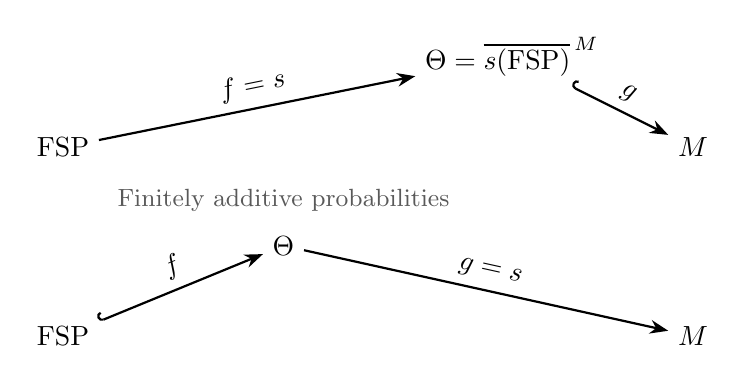
\begin{tikzpicture}[
			map/.style={-{Stealth}, thick},
			inclusion/.style={{Hooks[right]}-{Stealth}, thick},
			caption/.style={font=\small, text=black!65}
			]
			\node (fsp1) at (0,0) {$\FSP$};
			\node (theta1) at (5.7,1.15)
			{$\Theta=\overline{s(\FSP)}^{\,M}$};
			\node (m1) at (8,0) {$M$};
			
			\draw[map] (fsp1) -- node[above, sloped] {$f=s$} (theta1);
			\draw[inclusion] (theta1) -- node[above, sloped] {$g$} (m1);
			
			\node (fsp2) at (0,-2.4) {$\FSP$};
			\node (theta2) at (2.8,-1.25) {$\Theta$};
			\node[caption, above=2pt] at (theta2.north)
			{Finitely additive probabilities};
			\node (m2) at (8,-2.4) {$M$};
			
			\draw[inclusion] (fsp2) -- node[above, sloped] {$f$} (theta2);
			\draw[map] (theta2) -- node[above, sloped] {$g=s$} (m2);
		\end{tikzpicture}
	\end{center}
	
	A further choice is the pointwise closure of the finitely
	supported expectation functions in $[-\infty,\infty]^{\R^W}$.
	Here the inclusion sends $p$ to the function
	$X\mapsto\Exp_p(X)$ on real-valued gambles. Each coordinate is
	continuous on every finite simplex, and the closure is compact
	in the product topology.
\end{AIwritten}
\end{document}
\newpage
\color{red}
\part{DELETE}





\subsection{Coherent Admissibility for a different class}

\begin{conjecture}
	Suppose $\C$ is a class of models, with a topology. And suppose that the probabilities can be continuously embedded in $\C$, that is, there some continuous $s:P\to\C$\todo{that's always the case: just map them all to a single member of $\C$. Then the relevant sets will be closed.}. If $\succeq_w$ is generated by a continouous loss function on $\M$ where members of $\C$ are not strictly dominated. Then any $m\in \M\setminus \C$ are Pareto-dominated by, or have the same loss profile as, some member of $\C$. 
\end{conjecture}

No, this is false. It's important that the dominator is on the support. Otherwise we can just map them all to a single member of $\C$. 
Note that we certainly need
\[s(\delta_w)\succeq_w m^*\]


\subsection{Strictly proper scoring rules}
Suppose $L$ is a loss function on credence functions, possibily taking value $\infty$. 

Let $m'\succeq_w m$ when $L(m',w)\leq L(m,w)$. 

\begin{lemma}
	If $L$ is weakly proper, then \ref{ass:KKM} holds. 
	
	If $L$ is continuous, then \ref{ass:cl} holds.
	
	So, for a weakly proper continuous scoring rule, non-probabilities are Pareto-dominated by, or have the same loss profile as, a probability function. 
	
	If, in addition, $L$ is strictly proper, then every non-probability is actually Pareto-dominated. 
\end{lemma}

\begin{AIwritten}
	\subsection{Proper loss functions}
	
	Let $W$ be nonempty, and let $P$ be the finitely additive
	probabilities on $\wp(W)$, equipped with the topology
	of pointwise convergence on events. Let $M\supseteq P$
	be a set of credence functions, and let
	\[
	L\colon M\times W\to[0,\infty]
	\]
	be a loss function.
	
	We say that $L$ is \emph{proper} if
	\[
	E_p[L(p,\cdot)]\le E_p[L(m,\cdot)]
	\qquad(p\in P,\ m\in M),
	\]
	and \emph{strictly proper} if the inequality is strict
	whenever $m\neq p$.
	
	\begin{proposition}[Weak improvement under proper losses]
		Suppose $L$ is proper and:
		\begin{enumerate}
			\item For every finitely supported $p\in P$,
			\[
			E_p[L(p,\cdot)]<\infty.
			\]
			\item For every world $w$, the map
			$p\mapsto L(p,w)$ is lower semicontinuous.
		\end{enumerate}
		Then, for every $m\in M$, there is a probability
		$p\in P$ such that
		\[
		L(p,w)\le L(m,w)
		\qquad\text{for every }w\in W.
		\]
		The set of such probabilities is nonempty and compact.
		
		Consequently, every non-probabilistic report is
		either Pareto-dominated by a probability or has
		the same loss profile as a probability.
		
		If $L$ is strictly proper, every probability is
		Pareto-undominated, and every non-probabilistic
		report is Pareto-dominated by a probability.
	\end{proposition}
	
	\begin{proof}
		Apply the preceding corollary with $s(p)=p$ and
		\[
		m'\succeq_w m
		\quad\Longleftrightarrow\quad
		L(m',w)\le L(m,w).
		\]
		
		For closedness, fix $m$ and $w$. If $L(m,w)$
		is finite, the comparison set
		\[
		\{p:L(p,w)\le L(m,w)\}
		\]
		is closed by lower semicontinuity. If
		$L(m,w)=\infty$, the comparison set is all of $P$.
		
		For coherent admissibility, take a finitely
		supported $p$ and a benchmark $m$. If
		\[
		L(m,w)<L(p,w)
		\qquad\text{for every }w\in\supp(p),
		\]
		finite support and finite truthful expected loss
		would give
		\[
		E_p[L(m,\cdot)]<E_p[L(p,\cdot)],
		\]
		contradicting propriety. Hence some world in
		$\supp(p)$ satisfies $L(p,w)\le L(m,w)$.
		
		The corollary gives the required probability.
		Its possible witnesses form a closed subset
		of compact $P$, so that set is compact.
		
		Under strict propriety, no report distinct from
		a probability $p$ can weakly improve its loss
		everywhere: that would contradict
		\[
		E_p[L(p,\cdot)]<E_p[L(m,\cdot)].
		\]
		Thus every probability is Pareto-undominated.
		Likewise, a non-probabilistic benchmark cannot
		have the same loss profile as its probabilistic
		weak improver. The improvement must therefore
		be strict somewhere.
	\end{proof}
	
	\begin{proposition}[Uniform dominance with finitely many worlds]
		Suppose $W$ is finite, $L$ is strictly proper,
		and $L(p,w)$ is finite for every $p\in P$ and
		$w\in W$. Suppose also that $p\mapsto L(p,w)$
		is lower semicontinuous for every $w$.
		
		Let $m\in M\setminus P$ have finite loss at every
		world. Then there are $p^*\in P$ and $\nu>0$ such that
		\[
		L(p^*,w)\le L(m,w)-\nu
		\qquad\text{for every }w\in W.
		\]
		In particular, $m$ is uniformly strictly dominated
		by a Pareto-undominated probability.
	\end{proposition}
	
	\begin{proof}
		Define the optimal expected loss
		\[
		H(p)=E_p[L(p,\cdot)].
		\]
		Propriety gives
		\[
		H(p)=\inf_{q\in P}E_p[L(q,\cdot)].
		\]
		For each fixed $q$, its expected loss is continuous
		in $p$, since $W$ is finite and $L(q,w)$ is finite.
		Thus $H$ is upper semicontinuous.
		
		The expected advantage of $p$ over $m$ is
		\[
		D_m(p)=E_p[L(m,\cdot)]-H(p).
		\]
		It is lower semicontinuous, and strict propriety
		makes it strictly positive everywhere.
		Compactness of $P$ therefore gives
		\[
		\nu=\min_{p\in P}D_m(p)>0.
		\]
		
		For each world $w$, define
		\[
		\psi_m(w)=
		\{p\in P:L(p,w)\le L(m,w)-\nu\}.
		\]
		These sets are closed by lower semicontinuity.
		
		For every $p\in P$,
		\[
		\sum_{w\in\supp(p)}
		p(w)\bigl[L(m,w)-L(p,w)\bigr]\ge\nu.
		\]
		Hence some $w\in\supp(p)$ satisfies
		$L(p,w)\le L(m,w)-\nu$.
		This is the KKM covering condition.
		
		Fan--KKM supplies
		$p^*\in\bigcap_{w\in W}\psi_m(w)$,
		giving the stated uniform improvement.
		Strict propriety makes $p^*$ Pareto-undominated
		by the preceding proposition.
	\end{proof}
\end{AIwritten}



\section{Wald}

\begin{color}{blue}\begin{proposition}[Weak improvement by a Bayes option]
		Let $\Omega$ be finite and nonempty, let
		$\U\colon\mathcal O\times\Omega\to\mathbb R$,
		and let $P$ be the probability simplex on $\Omega$.
		Write $B(p)$ for the options Bayes for $p$.
		
		Suppose $B(p)\neq\varnothing$ for every $p\in P$,
		and that, for every benchmark $m$ and world $w$,
		the set
		\[
		\{p\in P:\U(o,w)\ge\U(m,w)
		\text{ for every }o\in B(p)\}
		\]
		is closed.
		
		Then every option is weakly improved upon at every
		world by a Bayes option. Moreover, every Bayes option
		is Pareto-undominated. Consequently, every non-Bayes
		option is Pareto-dominated by a Bayes option.
	\end{proposition}
	
	\begin{proof}
		First, all options Bayes for the same prior have
		identical utility profiles. Take $a,b\in B(p)$,
		fix $w$, and put
		\[
		p_n=(1-1/n)p+(1/n)\delta_w.
		\]
		For every $o\in B(p_n)$, Bayes optimality gives
		\[
		(1-1/n)\bigl[E_p\U(o)-E_p\U(b)\bigr]
		+\frac1n\bigl[\U(o,w)-\U(b,w)\bigr]\ge0.
		\]
		The first bracket is nonpositive, so
		$\U(o,w)\ge\U(b,w)$. By closedness, this holds
		for every $o\in B(p)$, including $a$.
		Interchanging $a$ and $b$ gives equality.
		
		Fix a benchmark $m$ and define
		\[
		\psi(w)=
		\{p\in P:\U(o,w)\ge\U(m,w)
		\text{ for every }o\in B(p)\}.
		\]
		These sets are closed. For each $p$, Bayes
		optimality gives some $w\in\supp(p)$ where
		a Bayes option performs at least as well as $m$.
		Since all Bayes options for $p$ have the same
		profile, $p\in\psi(w)$. Fan--KKM therefore gives
		a prior whose Bayes options weakly improve upon
		$m$ at every world.
		
		If an option $b$ weakly improves upon
		$a\in B(p)$ everywhere, then $b\in B(p)$.
		Profile equality forces them to tie everywhere.
		Thus every Bayes option is Pareto-undominated.
		
		Finally, a non-Bayes benchmark cannot tie everywhere
		with its Bayes weak improver, since that would make
		it Bayes for the same prior. It is therefore
		Pareto-dominated.
	\end{proof}
	
	\begin{proposition}[Uniform strict dominance]
		Assume the preceding hypotheses. Suppose additionally
		that, for every world $w$ and real threshold $r$,
		the set
		\[
		\{p\in P:\U(o,w)\ge r
		\text{ for every }o\in B(p)\}
		\]
		is closed.
		
		Then every non-Bayes option is uniformly strictly
		dominated by a Pareto-undominated Bayes option.
	\end{proposition}
	
	\begin{proof}
		Fix a non-Bayes option $m$. Define
		\[
		D_m(p)=
		\sup_{o\in\mathcal O}E_p[\U(o)-\U(m)].
		\]
		Bayes existence makes this supremum finite
		and attained. Since $m$ is never Bayes,
		$D_m(p)>0$ for every $p$.
		
		As a supremum of continuous functions of $p$,
		$D_m$ is lower semicontinuous. Compactness gives
		\[
		\nu=\min_{p\in P}D_m(p)>0.
		\]
		Define
		\[
		\psi_\nu(w)=
		\{p\in P:\U(o,w)\ge\U(m,w)+\nu
		\text{ for every }o\in B(p)\}.
		\]
		These sets are closed by the additional assumption.
		
		For every $p$, a Bayes option has expected
		advantage $D_m(p)\ge\nu$. Hence it improves
		upon $m$ by at least $\nu$ at some world
		in $\supp(p)$. All Bayes options for $p$
		have the same profile, so $p\in\psi_\nu(w)$.
		Fan--KKM gives a prior $p^*$ whose Bayes
		options satisfy
		\[
		\U(o,w)\ge\U(m,w)+\nu
		\qquad\text{for every }w\in\Omega.
		\]
		These options are Pareto-undominated by
		the preceding proposition.
	\end{proof}
\end{color}



\section{Families}


\begin{corollary}[Families of rankings]
	Let $W$ be a nonempty set, let $P$ be the space of
	finitely additive probabilities on $2^W$ with the
	topology of pointwise convergence on events, and
	let $\mathfrak L$ be a family of rankings.
	
	Each ranking $L$ has a nonempty domain $M_L$ and
	comparison relations $\succeq_w^L$ for $w\in W$.
	Suppose that, for each $L\in\mathfrak L$, there is
	a selection $c_L\colon P\to M_L$ satisfying:
	\begin{enumerate}
		\item For every $m\in M_L$ and $w\in W$, the set
		\[
		\{p\in P:c_L(p)\succeq_w^L m\}
		\]
		is closed.
		\item For every finitely supported $p\in P$
		and every $m\in M_L$, there is some
		$w\in\supp(p)$ such that
		\[
		c_L(p)\succeq_w^L m.
		\]
	\end{enumerate}
	Then, under each ranking $L$, every model in $M_L$
	is weakly dominated by a model in the range of $c_L$.
	
	Fix a class $C$ of coherent models, and write
	$U_L$ for the undominated models under $L$ and
	$C_L=C\cap U_L$.
	Suppose additionally that, for every $L$:
	\begin{enumerate}
		\item the range of $c_L$ is contained in $C_L$;
		\item $C_L$ is closed under ties at every world.
	\end{enumerate}
	Then $U_L=C_L$, and every model in $M_L\setminus C_L$
	is dominated by a member of $C_L$.
	
	If every model is evaluated by some ranking, and
	every coherent model belongs to $C_L$ for some $L$,
	the models undominated under at least one ranking
	that evaluates them are exactly the coherent models.
	Every incoherent model is dominated under every
	ranking that evaluates it.
\end{corollary}

\begin{proof}
	Fix $L$ and apply the preceding theorem to $c_L$.
	Every $m\in M_L$ is therefore weakly dominated by
	some $a$ in the range of $c_L$.
	
	Under the additional assumptions, $a\in C_L$.
	If $m$ is undominated, it must be tied at every
	world with $a$. Closure under ties gives $m\in C_L$.
	Hence $U_L\subseteq C_L$, and the reverse inclusion
	holds by definition.
	
	If $m\notin C_L$, it cannot be tied at every world
	with $a$, so $a$ dominates $m$.
	
	Consequently, any model undominated under some
	ranking is coherent. Conversely, every coherent
	model belongs to $C_L$ for some $L$ and is therefore
	undominated under that ranking.
\end{proof}



\end{document}
